\chapter{Testes e Simulações}

Para ilustrar o funcionamento dos algoritmos, foi proposta uma planta hidráulica composta por um sistema de tanques comunicantes. A figura \ref{fig:TanquesComunicantes} mostra um esboço de tal sistema. O tanque com capacitância $C_1$ é interligado com um de capacitância $C_2$. Aquele é alimentado por uma vazão $q$ e é drenado por uma vazão $q_1$. Tal grandeza é controlada por um registro, que pode ser enxergado como um resistor de resistência $R_1$.

Ainda, devido à ligação, a vazão de saída do primeiro tanque é a entrada do segundo. Este é drenado por uma vazão $q_2$, onde é controlado por um registro $R_2$. A variável controlada é a diferença $h_1 - h_2$.

\begin{figure}[!ht]
\centering
\usetikzlibrary{calc}
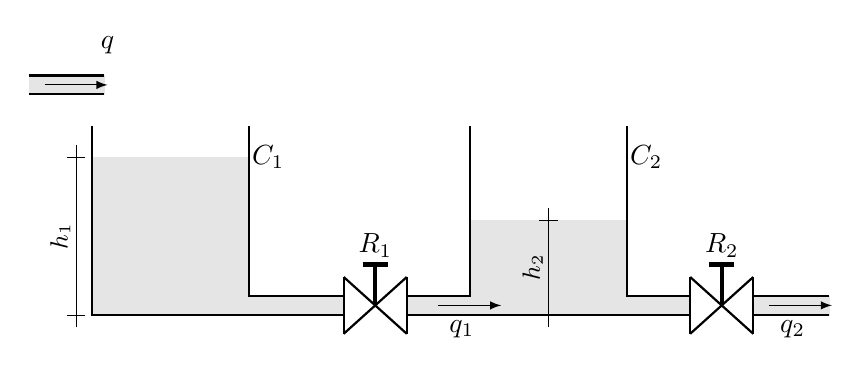
\begin{tikzpicture}[scale=0.8]
    \draw [ultra thin,color=Gray!20,fill] (0,-.5) rectangle (2.5,-3);
    \draw [ultra thin,color=Gray!20,fill] (2.5,-3) rectangle ++(1.5,.3);
    \draw [ultra thin,color=Gray!20,fill] (6,-1.5) rectangle (8.5,-3);
    \draw [ultra thin,color=Gray!20,fill] (10.5,-3) rectangle ++(1.2,.3);
    \draw [thick] (0,0) -- (0,-3) -- ++(4,0) coordinate(FimDoCano);
    \draw [thick] ($(FimDoCano)+(0,.3)$) -- ++(-1.5,0) -- ++(0,2.7);
    
    \draw [ultra thin,color=Gray!20,fill] ($(FimDoCano)+(1,0)$) rectangle ++(4.5,.3);
    \draw [thick] ($(FimDoCano)+(0,-.3)$) -- ++(0,.9);
    \draw [thick] ($(FimDoCano)+(0,-.3)$) -- ++(1,.9);
    \draw [thick] ($(FimDoCano)+(1,.6)$) -- ++(0,-.9);
    \draw [thick] ($(FimDoCano)+(1,-.3)$) -- ($(FimDoCano)+(0,.6)$);
    \draw [ultra thick] ($(FimDoCano)+(.5,.15)$) -- ++(0,.65) coordinate (Registro);
    \draw [ultra thick] ($(Registro)+(-.2,0)$) -- ($(Registro)+(.2,0)$);
    \draw [-latex] ($(FimDoCano)+(1.5,.15)$) -- ++(1,0) node [xshift=-.5cm,yshift=-.3cm] {$q_1$};
    \draw [thick] ($(FimDoCano)+(1,0)$) -- ++(4.5,0) ++(0,.3) -- ++(-1,0) -- ++(0,2.7) ++(-2.5,0) -- ++(0,-2.7) -- ++(-1,0);
    \draw [thick] ($(FimDoCano)+(5.5,-.3)$) -- ++(0,.9);
    \draw [thick] ($(FimDoCano)+(5.5,-.3)$) -- ++(1,.9);
    \draw [thick] ($(FimDoCano)+(6.5,.6)$) -- ++(0,-.9);
    \draw [thick] ($(FimDoCano)+(6.5,-.3)$) -- ($(FimDoCano)+(5.5,.6)$);
    \draw [ultra thick] ($(FimDoCano)+(6,.15)$) -- ++(0,.65) coordinate (Registro2);
    \draw [ultra thick] ($(Registro2)+(-.2,0)$) -- ($(Registro2)+(.2,0)$);\draw [very thin] (-.1,-3) -- ++(-.3,0);
    \draw [very thin] (-.1,-.5) -- ++(-.3,0);
    \draw [very thin] (-.25,-3.2) -- ++(0,2.9);
    \node [rotate=90] at (-.5,-1.75) {\small$h_1$};
    \draw [very thin] (7.4,-1.5) -- ++(-.3,0);
    \draw [very thin] (7.25,-3.2) -- ++(0,1.9);
    \node [rotate=90] at (7,-2.25) {\small$h_2$};
    \node (NomedoRegistro) at ($(Registro)+(0,.3)$) {$R_1$};
    \node (NomedoTanque) at ($(FimDoCano)+(-1.2,2.5)$) {$C_1$};
    \node (NomedoRegistro2) at ($(Registro2)+(0,.3)$) {$R_2$};
    \node (NomedoTanque2) at ($(FimDoCano)+(4.8,2.5)$) {$C_2$};
    \draw [ultra thin,color=Gray!20,fill] (-1,.5) rectangle ++(1.2,.3);
    \draw [thick] (-1,.5) -- ++(1.2,0) ++(0,.3) -- ++(-1.2,0);
    \draw [-latex] (-.75,.65) -- ++(1,0) node [yshift=.5cm] {$q$};
    \draw [thick] (10.5,-3) -- ++(1.2,0) ++(0,.3) -- ++(-1.2,0);
    \draw [-latex] (10.75,-2.85) -- ++(1,0) node [xshift=-.5cm,yshift=-.3cm] {$q_2$};
\end{tikzpicture}
\caption{Tanques comunicantes.}
\label{fig:TanquesComunicantes}
\end{figure}

\section{Modelagem via espaço de estados}
Para a representação via espaço de estados, define-se as variáveis de estado $x_1 = q_1$ e $x_2 = q_2$. A partir das relações entre capacitância e vazão, chega-se a seguinte representação no espaço de estados:
\begin{subequations}
\begin{align}
\dot{\pmb{\mathrm{x}}} &= \begin{bmatrix*}[c]
-(R_1C_{eq})^{-1} & (R_1C_2)^{-1}\\
(R_2C_2)^{-1} & -(R_2C_2)^{-1}
\end{bmatrix*}\pmb{\mathrm{x}} + \begin{bmatrix*}[c]
(R_1C_1)^{-1}\\
0
\end{bmatrix*}\pmb{\mathrm{u}}\label{eq:SSTCEntrada}\\
\pmb{\mathrm{y}} &= \begin{bmatrix*}[c]
R_1 & 0
\end{bmatrix*}\pmb{\mathrm{x}}\label{eq:SSTCSaida}
\end{align}
\end{subequations}
onde $C_{eq} = C_1C_2/(C_1 + C_2)$. Para discretizar o sistema, é preciso de um valor para o período de amostragem $T_s$. A transformada usada será a bilinear de Tustin, dada por:
\begin{equation}
\s = \dfrac{2}{T_s}\dfrac{\z-1}{\z+1}\label{eq:BilinearTransform}
\end{equation}
onde o semi-plano esquerdo dos contínuos é mapeado no círculo unitário dos discretos.

\section{Parâmetros de projeto}
Com posse do espaço de estados, é possível sintetizar uma matriz de ganho $K$ que possa estabilizar o sistema. Antes, é necessário atribuir valores para a planta. Sem perda de generalidade, serão escolhidas arbitrariamente tais valores, como segue:
\begin{itemize}
\item $C_1 = C_2 = 5$;
\item $R_1 = R_2 = 1$;
\item $T_s = \SI{10}{\second}$.
\end{itemize}

A período de amostragem escolhido possui valor elevado devido à dinâmica do sistema, que é na ordem de segundos ou até minutos. Assim, a representação via espaço de estados da planta nos contínuos é dada por:
\begin{subequations}
\begin{align}
\dot{\pmb{\mathrm{x}}} &= \begin{bmatrix*}[c]
-0,4 & -0,2\\
0,2 & -0,2
\end{bmatrix*}\pmb{\mathrm{x}} + \begin{bmatrix*}[c]
0,2\\
0
\end{bmatrix*}\pmb{\mathrm{u}}\label{eq:SSCTCEntrada}\\
\pmb{\mathrm{y}} &= \begin{bmatrix*}[c]
1 & 0
\end{bmatrix*}\pmb{\mathrm{x}}\label{eq:SSCTCSaida}
\end{align}
\end{subequations}

Através do função \texttt{c2d} disponibilizada no MATLAB$\copyright$\cite{MATLAB}, a transformação bilinear é realizada, resultando em:
\begin{subequations}
\begin{align}
\pmb{\mathrm{x^{+}}} &= \begin{bmatrix*}[c]
-0,4286 & -0,2857\\
0,2857 & -0,1429
\end{bmatrix*}\pmb{\mathrm{x}} + \begin{bmatrix*}[c]
0,5714\\
0,2857
\end{bmatrix*}\pmb{\mathrm{u}}\label{eq:SSDTCEntrada}\\
\pmb{\mathrm{y}} &= \begin{bmatrix*}[c]
0,2857 & -0,1426
\end{bmatrix*}\pmb{\mathrm{x}} + \begin{bmatrix*}[c]
0,2857
\end{bmatrix*}\pmb{\mathrm{u}}\label{eq:SSDTCSaida}
\end{align}
\end{subequations}

Após a transformação, a característica mais notável é a presença da matriz $D$: o surgimento de transmissão direta é uma consequência da transformação bilinear\cite{CHIQUETO2021}. Com posse das matrizes obtidas na representação via espaço de estados, é possível escolher os parâmetros de projeto:
\begin{itemize}
\item $t_s = \SI{50}{\second}$;
\item $\zeta = 0,5 \implies M_p \leq 0,16$;
\item $\omega_n = \SI{0,1}{\radian/\second}$.
\end{itemize}

Neste caso, o raio da circunferência relativo à estabilidade possui valor igual à $0,4493$. Ainda, a constante $N_y$ possui o valor de $6,2832$, acima do recomendado. Além disso, a maior frequência natural não-amortecida de malha aberta do sistema discretizado possui o valor igual a $0,3780\,\si{\radian/\second}$.

Ao executar o algoritmo utilizando a aproximação cônica, a solução proposta é infactível. Ao checar a os resíduos da solução, apenas houve uma infactibilidade em relação à taxa de amortecimento (o resíduo associado é negativo). Tal fenômeno é comum em solucionadores numéricos, uma vez que podem admitir uma certa infactibilidade. A figura \ref{subfig:TesteC} mostra o diagrama de pólos do sistema compensado. É possível notar que o sistema é estável, mesmo com a negativa do algoritmo.

\begin{figure}[!ht]
\centering
\begin{subfigure}[t]{0.3\columnwidth}
\input{figuras/pzmap_testeC.tikz}
\caption{}
\label{subfig:TesteC}
\end{subfigure}
\begin{subfigure}[t]{0.3\columnwidth}
\input{figuras/pzmap_testeE.tikz}
\caption{}
\label{subfig:TesteE}
\end{subfigure}
\begin{subfigure}[t]{0.3\columnwidth}
% This file was created by matlab2tikz.
%
%The latest updates can be retrieved from
%  http://www.mathworks.com/matlabcentral/fileexchange/22022-matlab2tikz-matlab2tikz
%where you can also make suggestions and rate matlab2tikz.
%
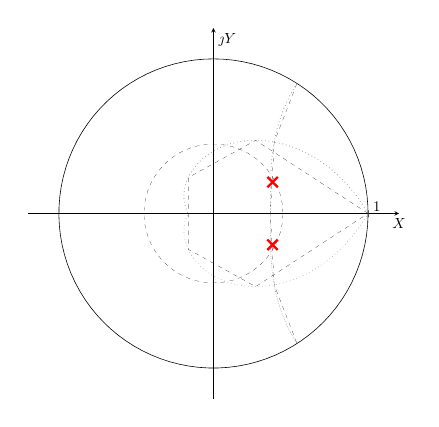
\begin{tikzpicture}[scale=0.53]

\begin{axis}[%
  axis lines=center,
  width=3.5in,
  height=3.5in,
  scale only axis,
  unbounded coords=jump,
  xmin=-1.2,
  xmax=1.2,
  ymin=-1.2,
  ymax=1.2,
  xtick={1},
  ytick=\empty,
  xticklabel style={anchor=south west, draw=none},
  xlabel={$X$},
  ylabel={$\jmath Y$},
  x label style={anchor=north}
]
\addplot [color=black!40, dotted, forget plot]
  table[row sep=crcr]{%
1	0\\
0.994975166457918	0.0086169531277774\\
0.989901329986755	0.0171473087453408\\
0.98477948302476	0.0255910797348211\\
0.979610612912339	0.0339482874654127\\
0.97439570184454	0.0422189617067992\\
0.96913572682452	0.0504031405426052\\
0.963831659617994	0.0585008702838818\\
0.958484466708655	0.0665122053826345\\
0.953095109254565	0.0744372083454012\\
0.947664543045514	0.0822759496468887\\
0.942193718461326	0.0900285076436762\\
0.936683580431134	0.0976949684879922\\
0.931135068393585	0.105275426041575\\
0.925549116258005	0.112769981789622\\
0.919926652366486	0.120178744754836\\
0.914268599456912	0.127501831411582\\
0.90857587462691	0.134739365600147\\
0.902849389298715	0.14189147844113\\
0.89709004918496	0.148958308249953\\
0.891298754255365	0.155940000451509\\
0.88547639870433	0.162836707494953\\
0.879623870919433	0.169648588768638\\
0.873742053450808	0.176375810515214\\
0.867831822981418	0.183018545746879\\
0.8618940502982	0.189576974160811\\
0.855929600264091	0.196051282054771\\
0.849939331790917	0.202441662242887\\
0.843924097813143	0.208748313971631\\
0.837884745262484	0.214971442835991\\
0.831822115043362	0.221111260695846\\
0.825737042009206	0.227167985592546\\
0.819630354939596	0.233141841665717\\
0.81350287651823	0.23903305907027\\
0.807355423311723	0.244841873893657\\
0.801188805749226	0.250568528073344\\
0.795003828102853	0.256213269314532\\
0.78880128846892	0.26177635100812\\
0.782581978749986	0.267258032148917\\
0.776346684637685	0.272658577254117\\
0.770096185596349	0.277978256282022\\
0.763831254847411	0.283217344551051\\
0.757552659354593	0.288376122659003\\
0.751261159809852	0.293454876402612\\
0.744957510620097	0.298453896697378\\
0.738642459894664	0.303373479497687\\
0.732316749433537	0.308213925717227\\
0.725981114716321	0.312975541149701\\
0.719636284891949	0.317658636389843\\
0.71328298276912	0.322263526754741\\
0.706921924807467	0.326790532205477\\
0.700553821109446	0.331239977269081\\
0.694179375412927	0.335612190960806\\
0.687799285084511	0.339907506706737\\
0.681414241113527	0.344126262266724\\
0.675024928106738	0.34826879965765\\
0.668632024283728	0.352335465077047\\
0.662236201472974	0.356326608827046\\
0.65583812510859	0.360242585238686\\
0.649438454227737	0.364083752596562\\
0.643037841468706	0.367850473063845\\
0.636636933069644	0.371543112607646\\
0.630236368867939	0.375162040924758\\
0.623836782300241	0.378707631367759\\
0.617438800403127	0.382180260871485\\
0.611043043814387	0.385580309879881\\
0.604650126774944	0.388908162273233\\
0.598260657131382	0.392164205295778\\
0.591875236339095	0.395348829483698\\
0.585494459466028	0.398462428593512\\
0.579118915197029	0.401505399530848\\
0.572749185838786	0.40447814227962\\
0.566385847325349	0.4073810598316\\
0.560029469224235	0.410214558116388\\
0.553680614743102	0.412979045931794\\
0.547339840736992	0.415674934874619\\
0.541007697716132	0.418302639271854\\
0.534684729854293	0.420862576112287\\
0.528371474997687	0.423355164978523\\
0.522068464674416	0.425780827979435\\
0.515776224104452	0.428139989683019\\
0.509495272210138	0.430433077049683\\
0.503226121627222	0.432660519365961\\
0.496969278716402	0.434822748178651\\
0.490725243575377	0.436920197229388\\
0.484494510051408	0.438953302389643\\
0.478277565754372	0.440922501596166\\
0.472074892070308	0.44282823478686\\
0.465886964175444	0.444670943837092\\
0.459714251050707	0.446451072496453\\
0.453557215496707	0.448169066325949\\
0.447416314149175	0.449825372635651\\
0.441291997494877	0.451420440422779\\
0.435184709887969	0.452954720310238\\
0.429094889566804	0.454428664485608\\
0.423022968671182	0.455842726640584\\
0.416969373260031	0.457197361910859\\
0.410934523329524	0.458493026816478\\
0.404918832831608	0.459730179202636\\
0.398922709692961	0.460909278180935\\
0.392946555834355	0.462030784071105\\
0.386990767190422	0.463095158343177\\
0.381055733729824	0.46410286356012\\
0.375141839475811	0.465054363320948\\
0.369249462527169	0.465950122204273\\
0.363378975079551	0.466790605712337\\
0.357530743447174	0.467576280215505\\
0.351705128084897	0.46830761289722\\
0.345902483610657	0.468985071699428\\
0.34012315882826	0.469609125268472\\
0.334367496750526	0.47018024290145\\
0.328635834622783	0.470698894493046\\
0.322928503946697	0.471165550482829\\
0.317245830504437	0.471580681803022\\
0.311588134383171	0.471944759826739\\
0.305955729999881	0.472258256316704\\
0.300348926126498	0.472521643374422\\
0.294768025915352	0.472735393389845\\
0.289213326924917	0.47289997899149\\
0.283685121145871	0.473015872997045\\
0.278183695027438	0.473083548364434\\
0.272709329504025	0.473103478143368\\
0.267262300022144	0.473076135427362\\
0.261842876567611	0.473001993306221\\
0.256451323693014	0.472881524819009\\
0.251087900545453	0.472715202907487\\
0.24575286089454	0.472503500370018\\
0.240446453160655	0.472246889815953\\
0.235168920443456	0.471945843620488\\
0.229920500550629	0.471600833879988\\
0.224701426026886	0.471212332367794\\
0.219511924183188	0.470780810490488\\
0.214352217126212	0.470306739244642\\
0.209222521788028	0.46979058917403\\
0.204123049956005	0.469232830327317\\
0.199054008302929	0.468633932216212\\
0.194015598417329	0.467994363774097\\
0.189008016834009	0.467314593315119\\
0.184031455064777	0.466595088493758\\
0.179086099629367	0.465836316264853\\
0.174172132086558	0.465038742844109\\
0.169289729065466	0.464202833669053\\
0.16443906229702	0.463329053360474\\
0.159620298645616	0.462417865684317\\
0.154833600140936	0.461469733514039\\
0.150079124009928	0.460485118793442\\
0.145357022708955	0.45946448249995\\
0.140667443956089	0.458408284608366\\
0.136010530763565	0.457316984055071\\
0.131386421470369	0.456191038702701\\
0.126795249774977	0.455030905305267\\
0.122237144768225	0.453837039473741\\
0.117712230966311	0.452609895642096\\
0.113220628343922	0.451349927033798\\
0.108762452367488	0.450057585628759\\
0.104337814028549	0.448733322130736\\
0.0999468198772385	0.447377585935182\\
0.0955895720558732	0.445990825097552\\
0.0912661683326492	0.444573486302051\\
0.0869767021354367	0.443126014830835\\
0.0827212625856707	0.441648854533653\\
0.0784999345323338	0.440142447797942\\
0.0743127985860244	0.438607235519351\\
0.0701599311531092	0.437043657072723\\
0.0660414044699528	0.435452150283505\\
0.0619572866372231	0.433833151399599\\
0.0579076416542657	0.432187095063656\\
0.0538925294535447	0.4305144142858\\
0.0499120059351455	0.428815540416786\\
0.045966123001336	0.42709090312159\\
0.0420549285911806	0.425340930353435\\
0.0381784667152051	0.423566048328237\\
0.0343367774901069	0.421766681499485\\
0.0305298971735083	0.419943252533545\\
0.0267578581987466	0.418096182285383\\
0.0230206892096994	0.416225889774718\\
0.0193184150956407	0.414332792162584\\
0.0156510570261221	0.412417304728323\\
0.0120186324858799	0.410479840846984\\
0.00842115530975893	0.408520811967138\\
0.00485863571765306	0.406540627589113\\
0.00133108034945763	0.404539695243628\\
-0.00216150769996924	0.402518420470845\\
-0.00561912884584125	0.400477206799821\\
-0.00904178697847668	0.39841645572837\\
-0.0124294894283334	0.396336566703324\\
-0.0157822469310498	0.394237937101194\\
-0.0191000735924938	0.39212096220923\\
-0.0223829868538259	0.389986035206885\\
-0.0256310074565762	0.387833547147654\\
-0.028844159407742	0.385663886941331\\
-0.0320224699449067	0.383477441336632\\
-0.035165969501385	0.381274594904221\\
-0.0382746916713966	0.379055730020116\\
-0.0413486731752722	0.37682122684948\\
-0.044387953824694	0.374571463330791\\
-0.0473925764879758	0.372306815160395\\
-0.0503625870553824	0.37002765577743\\
-0.053298034404496	0.367734356349131\\
-0.0561989703656271	0.365427285756506\\
-0.0590654496872782	0.363106810580375\\
-0.0618975300016593	0.360773295087786\\
-0.0646952717902602	0.358427101218792\\
-0.0674587383494818	0.356068588573591\\
-0.0701879957563293	0.353698114400028\\
-0.0728831128341696	0.351316033581455\\
-0.0755441611185572	0.348922698624945\\
-0.078171214823129	0.346518459649865\\
-0.080764350805573	0.344103664376793\\
-0.083323648533672	0.341678658116792\\
-0.0858491900514256	0.339243783761024\\
-0.0883410599452533	0.336799381770708\\
-0.0907993453102799	0.334345790167427\\
-0.0932241357167081	0.331883344523768\\
-0.0956155231762785	0.329412377954299\\
-0.0979736021088205	0.326933221106879\\
-0.100298469308897	0.324446202154309\\
-0.102590223912543	0.3219516467863\\
-0.104848967364106	0.319449878201778\\
-0.107074803383181	0.316941217101503\\
-0.109267837931654	0.314425981681024\\
-0.111428179180845	0.311904487623941\\
-0.113555937478763	0.309377048095487\\
-0.115651225317466	0.306843973736431\\
-0.117714157300535	0.304305572657284\\
-0.119744850110663	0.301762150432819\\
-0.121743422477352	0.299214010096897\\
-0.12370999514474	0.296661452137599\\
-0.125644690839534	0.294104774492655\\
-0.127547634239077	0.29154427254518\\
-0.129418951939533	0.288980239119696\\
-0.131258772424195	0.286412964478459\\
-0.133067226031924	0.283842736318072\\
-0.13484444492572	0.281269839766384\\
-0.136590563061418	0.278694557379684\\
-0.138305716156522	0.27611716914017\\
-0.139990041659173	0.273537952453705\\
-0.141643678717248	0.27095718214785\\
-0.143266768147609	0.268375130470173\\
-0.144859452405477	0.26579206708683\\
-0.146421875553965	0.263208259081419\\
-0.147954183233735	0.260623970954104\\
-0.149456522632818	0.258039464621\\
-0.150929042456566	0.255454999413824\\
-0.152371892897761	0.252870832079808\\
-0.153785225606871	0.250287216781869\\
-0.155169193662457	0.24770440509903\\
-0.156523951541726	0.245122646027102\\
-0.157849655091252	0.242542185979612\\
-0.159146461497839	0.239963268788975\\
-0.160414529259544	0.237386135707918\\
-0.161654018156862	0.234811025411143\\
-0.162865089224069	0.232238173997232\\
-0.164047904720716	0.229667814990784\\
-0.165202628103302	0.227100179344793\\
-0.166329423997092	0.224535495443257\\
-0.167428458168113	0.221973989104012\\
-0.168499897495306	0.219415883581802\\
-0.169543909942848	0.216861399571562\\
-0.170560664532644	0.214310755211935\\
-0.171550331316981	0.211764166088996\\
-0.172513081351356	0.209221845240208\\
-0.173449086667475	0.206684003158576\\
-0.174358520246424	0.204150847797023\\
-0.175241555992005	0.201622584572976\\
-0.176098368704256	0.199099416373151\\
-0.176929134053141	0.196581543558548\\
-0.177734028552409	0.194069163969646\\
-0.178513229533643	0.191562472931801\\
-0.179266915120471	0.189061663260829\\
-0.179995264202967	0.1865669252688\\
-0.180698456412218	0.184078446770007\\
-0.181376672095087	0.181596413087137\\
-0.182030092289137	0.17912100705762\\
-0.18265889869775	0.176652409040165\\
-0.183263273665422	0.17419079692148\\
-0.183843400153239	0.171736346123169\\
-0.184399461714537	0.169289229608803\\
-0.184931642470749	0.16684961789117\\
-0.185440127087425	0.164417679039694\\
-0.185925100750451	0.161993578688022\\
-0.186386749142441	0.159577480041785\\
-0.18682525841932	0.157169543886511\\
-0.18724081518709	0.154769928595712\\
-0.18763360647879	0.152378790139125\\
-0.18800381973163	0.149996282091108\\
-0.188351642764323	0.147622555639199\\
-0.1886772637546	0.145257759592815\\
-0.188980871216915	0.142902040392114\\
-0.189262653980335	0.140555542116997\\
-0.189522801166623	0.138218406496255\\
-0.189761502168506	0.135890772916862\\
-0.189978946628136	0.133572778433407\\
-0.190175324415737	0.131264557777667\\
-0.190350825608445	0.128966243368309\\
-0.190505640469335	0.126677965320734\\
-0.19063995942664	0.124399851457046\\
-0.190753973053159	0.122132027316154\\
-0.19084787204586	0.119874616163997\\
-0.190921847205665	0.117627739003896\\
-0.190976089417432	0.11539151458703\\
-0.191010789630132	0.113166059423026\\
-0.191026138837202	0.110951487790669\\
-0.191022328057108	0.108747911748734\\
-0.190999548314082	0.106555441146921\\
-0.190957990619064	0.104374183636905\\
-0.190897845950822	0.1022042446835\\
-0.190819305237275	0.100045727575919\\
-0.190722559336998	0.0978987334391491\\
-0.190607799020923	0.0957633612454201\\
-0.190475214954231	0.0936397078257795\\
-0.190324997678427	0.0915278678817618\\
-0.190157337593618	0.0894279339971549\\
-0.189972424940972	0.0873399966498598\\
-0.18977044978537	0.0852641442238417\\
-0.18955160199825	0.083200463021171\\
-0.189316071240637	0.0811490372741514\\
-0.189064046946367	0.0791099491575331\\
-0.1887957183055	0.0770832788008092\\
-0.18851127424792	0.0750691043005936\\
-0.18821090342712	0.073067501733078\\
-0.187894794204192	0.0710785451665654\\
-0.187563134631983	0.0691023066740791\\
-0.187216112439458	0.0671388563460452\\
-0.186853915016241	0.065188262303045\\
-0.186476729397344	0.0632505907086381\\
-0.186084742248091	0.0613259057822507\\
-0.185678139849218	0.0594142698121313\\
-0.185257108082164	0.0575157431683673\\
-0.184821832414555	0.0556303843159656\\
-0.18437249788586	0.0537582498279896\\
-0.183909289093245	0.0518993943987567\\
-0.183432390177603	0.0500538708570886\\
-0.182941984809774	0.0482217301796184\\
-0.182438256176944	0.0464030215041461\\
-0.181921386969236	0.044597792143048\\
-0.18139155936647	0.0428060875967306\\
-0.180848955025119	0.041027951567134\\
-0.180293755065441	0.0392634259712775\\
-0.179726140058791	0.0375125509548501\\
-0.179146290015116	0.0357753649058401\\
-0.178554384370631	0.0340519044682056\\
-0.177950601975674	0.032342204555581\\
-0.177335121082737	0.0306462983650213\\
-0.176708119334683	0.0289642173907774\\
-0.176069773753131	0.0272959914381074\\
-0.175420260727028	0.0256416486371157\\
-0.174759756001391	0.0240012154566223\\
-0.174088434666228	0.0223747167180594\\
-0.173406471145636	0.0207621756093928\\
-0.172714039187066	0.0191636136990689\\
-0.172011311850774	0.0175790509499823\\
-0.171298461499436	0.0160085057334652\\
-0.170575659787937	0.0144519948432961\\
-0.16984307765334	0.0129095335097251\\
-0.169100885305011	0.0113811354135165\\
-0.168349252214934	0.00986681270000477\\
-0.167588347108177	0.00836657599316387\\
-0.166818337953539	0.00688043440968819\\
-0.166039391954362	0.00540839557308299\\
-0.165251675539513	0.00395046562776311\\
-0.164455354354524	0.00250664925315921\\
-0.163650593252911	0.00107694967782874\\
};

\addplot [color=black!40, dotted, forget plot, each nth point=10]
  table[row sep=crcr]{%
0.54030230586814	0.841470984807897\\
0.539762693938401	0.840629664537062\\
0.539224460721023	0.83978864621053\\
0.53868760316101	0.838947930597949\\
0.538152118209836	0.838107518462474\\
0.537618002825427	0.837267410560788\\
0.537085253972145	0.836427607643129\\
0.53655386862078	0.835588110453312\\
0.536023843748535	0.83474891972876\\
0.535495176339009	0.833910036200521\\
0.534967863382191	0.833071460593297\\
0.534441901874438	0.832233193625467\\
0.533917288818469	0.831395236009111\\
0.533394021223349	0.830557588450033\\
0.532872096104475	0.829720251647789\\
0.532351510483565	0.828883226295704\\
0.531832261388641	0.828046513080903\\
0.531314345854023	0.827210112684328\\
0.530797760920307	0.826374025780767\\
0.53028250363436	0.825538253038873\\
0.529768571049302	0.82470279512119\\
0.529255960224495	0.823867652684175\\
0.528744668225529	0.823032826378221\\
0.52823469212421	0.822198316847678\\
0.527726028998549	0.821364124730882\\
0.527218675932742	0.820530250660169\\
0.526712630017168	0.819696695261905\\
0.526207888348365	0.818863459156502\\
0.525704448029027	0.818030542958447\\
0.525202306167984	0.817197947276319\\
0.524701459880193	0.816365672712812\\
0.524201906286724	0.815533719864761\\
0.523703642514747	0.814702089323156\\
0.523206665697522	0.813870781673172\\
0.522710972974383	0.813039797494186\\
0.522216561490726	0.8122091373598\\
0.521723428397999	0.811378801837861\\
0.521231570853687	0.810548791490484\\
0.5207409860213	0.809719106874073\\
0.520251671070359	0.808889748539341\\
0.519763623176388	0.808060717031331\\
0.519276839520897	0.80723201288944\\
0.518791317291371	0.806403636647435\\
0.518307053681259	0.805575588833477\\
0.51782404588996	0.80474786997014\\
0.517342291122811	0.803920480574434\\
0.516861786591075	0.803093421157821\\
0.516382529511928	0.802266692226238\\
0.515904517108448	0.80144029428012\\
0.515427746609602	0.800614227814413\\
0.514952215250233	0.799788493318601\\
0.514477920271049	0.79896309127672\\
0.514004858918611	0.798138022167384\\
0.51353302844532	0.797313286463798\\
0.513062426109404	0.796488884633783\\
0.512593049174908	0.795664817139792\\
0.512124894911682	0.794841084438931\\
0.511657960595367	0.794017686982978\\
0.511192243507383	0.793194625218402\\
0.510727740934919	0.792371899586382\\
0.510264450170919	0.791549510522827\\
0.509802368514074	0.790727458458392\\
0.509341493268803	0.7899057438185\\
0.508881821745247	0.789084367023359\\
0.508423351259256	0.788263328487982\\
0.507966079132375	0.787442628622202\\
0.507510002691835	0.786622267830696\\
0.507055119270539	0.785802246512997\\
0.506601426207052	0.784982565063518\\
0.506148920845586	0.784163223871566\\
0.505697600535993	0.78334422332136\\
0.505247462633751	0.782525563792053\\
0.504798504499949	0.781707245657746\\
0.504350723501283	0.780889269287506\\
0.503904117010036	0.780071635045386\\
0.503458682404072	0.779254343290439\\
0.503014417066823	0.77843739437674\\
0.502571318387277	0.777620788653398\\
0.502129383759965	0.776804526464577\\
0.501688610584954	0.775988608149514\\
0.501248996267831	0.775173034042531\\
0.500810538219691	0.774357804473059\\
0.500373233857132	0.773542919765647\\
0.499937080602236	0.772728380239986\\
0.499502075882562	0.771914186210922\\
0.499068217131134	0.771100337988471\\
0.498635501786428	0.770286835877842\\
0.498203927292362	0.769473680179445\\
0.497773491098285	0.768660871188913\\
0.497344190658966	0.767848409197119\\
0.49691602343458	0.767036294490186\\
0.496488986890701	0.766224527349511\\
0.496063078498286	0.765413108051773\\
0.495638295733668	0.764602036868957\\
0.495214636078543	0.763791314068363\\
0.49479209701996	0.762980939912625\\
0.494370676050306	0.762170914659728\\
0.493950370667301	0.761361238563018\\
0.493531178373981	0.760551911871226\\
0.493113096678692	0.759742934828473\\
0.492696123095076	0.758934307674296\\
0.49228025514206	0.758126030643656\\
0.491865490343845	0.757318103966953\\
0.491451826229899	0.756510527870047\\
0.491039260334939	0.755703302574268\\
0.490627790198926	0.754896428296429\\
0.490217413367051	0.754089905248849\\
0.489808127389725	0.753283733639359\\
0.48939992982257	0.75247791367132\\
0.488992818226405	0.751672445543641\\
0.488586790167236	0.750867329450786\\
0.488181843216247	0.750062565582796\\
0.487777974949788	0.749258154125298\\
0.487375182949364	0.748454095259521\\
0.486973464801624	0.747650389162311\\
0.486572818098353	0.746847036006143\\
0.486173240436456	0.746044035959138\\
0.485774729417954	0.745241389185073\\
0.485377282649968	0.744439095843398\\
0.484980897744711	0.743637156089248\\
0.484585572319477	0.742835570073457\\
0.484191303996629	0.742034337942574\\
0.483798090403591	0.74123345983887\\
0.483405929172836	0.740432935900359\\
0.483014817941875	0.739632766260805\\
0.482624754353249	0.738832951049743\\
0.482235736054514	0.738033490392481\\
0.481847760698234	0.737234384410123\\
0.481460825941973	0.736435633219578\\
0.481074929448277	0.735637236933574\\
0.480690068884672	0.734839195660667\\
0.480306241923647	0.734041509505259\\
0.479923446242647	0.733244178567608\\
0.479541679524064	0.732447202943843\\
0.479160939455223	0.73165058272597\\
0.478781223728375	0.730854318001894\\
0.478402530040683	0.730058408855422\\
0.478024856094217	0.729262855366284\\
0.477648199595939	0.728467657610137\\
0.477272558257696	0.727672815658583\\
0.476897929796208	0.726878329579179\\
0.476524311933058	0.726084199435447\\
0.476151702394684	0.725290425286892\\
0.475780098912366	0.724497007189005\\
0.475409499222216	0.723703945193283\\
0.475039901065173	0.722911239347235\\
0.474671302186985	0.722118889694397\\
0.474303700338206	0.721326896274341\\
0.47393709327418	0.720535259122689\\
0.473571478755038	0.719743978271122\\
0.473206854545681	0.718953053747392\\
0.472843218415775	0.718162485575335\\
0.472480568139739	0.71737227377488\\
0.472118901496735	0.716582418362059\\
0.471758216270658	0.715792919349022\\
0.47139851025013	0.715003776744045\\
0.471039781228482	0.71421499055154\\
0.470682027003753	0.713426560772069\\
0.470325245378674	0.712638487402353\\
0.469969434160663	0.71185077043528\\
0.46961459116181	0.71106340985992\\
0.469260714198871	0.710276405661534\\
0.468907801093259	0.709489757821582\\
0.46855584967103	0.708703466317736\\
0.468204857762879	0.70791753112389\\
0.467854823204124	0.707131952210168\\
0.467505743834703	0.706346729542938\\
0.467157617499157	0.705561863084818\\
0.46681044204663	0.704777352794687\\
0.46646421533085	0.703993198627698\\
0.466118935210123	0.703209400535282\\
0.465774599547328	0.702425958465164\\
0.465431206209898	0.701642872361368\\
0.46508875306982	0.700860142164228\\
0.46474723800362	0.700077767810399\\
0.464406658892354	0.699295749232865\\
0.464067013621601	0.698514086360948\\
0.463728300081451	0.697732779120317\\
0.463390516166498	0.696951827433\\
0.463053659775829	0.69617123121739\\
0.462717728813013	0.695390990388255\\
0.462382721186096	0.694611104856748\\
0.462048634807588	0.693831574530415\\
0.461715467594456	0.693052399313204\\
0.461383217468113	0.692273579105474\\
0.46105188235441	0.691495113804002\\
0.460721460183626	0.690717003301996\\
0.460391948890459	0.689939247489099\\
0.460063346414016	0.6891618462514\\
0.459735650697807	0.68838479947144\\
0.459408859689731	0.687608107028223\\
0.459082971342071	0.686831768797225\\
0.458757983611482	0.686055784650399\\
0.458433894458983	0.685280154456184\\
0.45811070184995	0.684504878079514\\
0.457788403754102	0.683729955381828\\
0.457466998145497	0.682955386221072\\
0.457146483002521	0.682181170451714\\
0.456826856307877	0.681407307924745\\
0.45650811604858	0.680633798487693\\
0.456190260215944	0.679860641984627\\
0.455873286805575	0.679087838256163\\
0.455557193817364	0.678315387139476\\
0.455241979255474	0.677543288468305\\
0.454927641128334	0.676771542072959\\
0.454614177448629	0.676000147780328\\
0.454301586233291	0.675229105413887\\
0.453989865503491	0.674458414793703\\
0.45367901328463	0.673688075736445\\
0.453369027606329	0.672918088055388\\
0.453059906502422	0.672148451560422\\
0.452751648010945	0.671379166058059\\
0.452444250174131	0.670610231351436\\
0.452137711038396	0.669841647240328\\
0.451832028654334	0.669073413521148\\
0.451527201076709	0.668305529986959\\
0.451223226364442	0.667537996427477\\
0.450920102580607	0.666770812629081\\
0.45061782779242	0.666003978374815\\
0.45031640007123	0.665237493444396\\
0.450015817492511	0.664471357614223\\
0.449716078135855	0.663705570657378\\
0.449417180084962	0.662940132343639\\
0.449119121427628	0.662175042439477\\
0.448821900255744	0.66141030070807\\
0.448525514665281	0.660645906909305\\
0.448229962756284	0.659881860799785\\
0.447935242632865	0.659118162132834\\
0.44764135240319	0.658354810658502\\
0.447348290179475	0.657591806123574\\
0.447056054077976	0.65682914827157\\
0.44676464221898	0.656066836842755\\
0.446474052726798	0.655304871574145\\
0.446184283729755	0.654543252199506\\
0.445895333360182	0.653781978449367\\
0.445607199754407	0.65302105005102\\
0.445319881052752	0.652260466728527\\
0.445033375399515	0.651500228202724\\
0.444747680942969	0.650740334191229\\
0.444462795835354	0.649980784408442\\
0.444178718232864	0.649221578565555\\
0.443895446295641	0.648462716370551\\
0.443612978187767	0.647704197528215\\
0.443331312077259	0.646946021740133\\
0.443050446136053	0.6461881887047\\
0.442770378540003	0.645430698117124\\
0.44249110746887	0.644673549669429\\
0.442212631106314	0.643916743050459\\
0.441934947639884	0.643160277945886\\
0.441658055261015	0.64240415403821\\
0.441381952165015	0.641648371006764\\
0.441106636551058	0.64089292852772\\
0.440832106622177	0.640137826274091\\
0.440558360585258	0.639383063915734\\
0.440285396651025	0.638628641119359\\
0.44001321303404	0.637874557548525\\
0.43974180795269	0.63712081286365\\
0.439471179629181	0.636367406722011\\
0.439201326289529	0.63561433877775\\
0.438932246163553	0.634861608681876\\
0.438663937484865	0.634109216082268\\
0.438396398490867	0.633357160623679\\
0.438129627422738	0.632605441947739\\
0.437863622525426	0.631854059692959\\
0.437598382047645	0.631103013494734\\
0.437333904241863	0.630352302985342\\
0.437070187364295	0.629601927793954\\
0.436807229674897	0.628851887546632\\
0.436545029437354	0.628102181866332\\
0.436283584919079	0.627352810372908\\
0.436022894391196	0.626603772683115\\
0.435762956128542	0.625855068410611\\
0.435503768409653	0.625106697165959\\
0.435245329516757	0.624358658556628\\
0.434987637735768	0.623610952186999\\
0.434730691356278	0.622863577658366\\
0.434474488671548	0.622116534568935\\
0.434219027978502	0.621369822513831\\
0.433964307577718	0.620623441085097\\
0.433710325773422	0.619877389871695\\
0.433457080873477	0.619131668459512\\
0.433204571189379	0.618386276431358\\
0.43295279503625	0.617641213366968\\
0.432701750732826	0.616896478843007\\
0.432451436601452	0.616152072433068\\
0.432201850968076	0.615407993707675\\
0.431952992162239	0.614664242234284\\
0.431704858517069	0.613920817577285\\
0.431457448369273	0.613177719298002\\
0.431210760059128	0.612434946954695\\
0.430964791930477	0.611692500102562\\
0.430719542330718	0.610950378293739\\
0.4304750096108	0.610208581077301\\
0.430231192125212	0.609467107999262\\
0.429988088231978	0.608725958602578\\
0.429745696292648	0.607985132427146\\
0.429504014672294	0.607244629009805\\
0.429263041739498	0.606504447884337\\
0.429022775866347	0.605764588581468\\
0.428783215428427	0.605025050628865\\
0.428544358804814	0.604285833551141\\
0.428306204378065	0.603546936869854\\
0.428068750534215	0.602808360103502\\
0.427831995662766	0.602070102767534\\
0.427595938156682	0.601332164374336\\
0.427360576412381	0.600594544433245\\
0.427125908829728	0.599857242450537\\
0.426891933812026	0.599120257929434\\
0.426658649766011	0.598383590370103\\
0.426426055101846	0.59764723926965\\
0.426194148233109	0.596911204122128\\
0.425962927576792	0.596175484418529\\
0.425732391553288	0.595440079646789\\
0.425502538586388	0.594704989291781\\
0.425273367103272	0.59397021283532\\
0.425044875534504	0.593235749756162\\
0.424817062314021	0.592501599529995\\
0.42458992587913	0.59176776162945\\
0.424363464670499	0.59103423552409\\
0.424137677132149	0.590301020680412\\
0.42391256171145	0.589568116561847\\
0.423688116859112	0.58883552262876\\
0.423464341029178	0.58810323833844\\
0.423241232679015	0.587371263145111\\
0.423018790269314	0.586639596499918\\
0.422797012264074	0.585908237850935\\
0.422575897130603	0.585177186643157\\
0.422355443339504	0.584446442318501\\
0.422135649364675	0.583716004315801\\
0.421916513683297	0.582985872070811\\
0.421698034775829	0.582256045016197\\
0.421480211126001	0.581526522581538\\
0.421263041220808	0.580797304193323\\
0.421046523550503	0.58006838927495\\
0.420830656608586	0.579339777246718\\
0.420615438891806	0.578611467525831\\
0.420400868900144	0.577883459526392\\
0.420186945136815	0.5771557526594\\
0.419973666108256	0.576428346332746\\
0.41976103032412	0.575701239951214\\
0.419549036297272	0.574974432916473\\
0.419337682543778	0.574247924627077\\
0.419126967582901	0.57352171447846\\
0.418916889937096	0.572795801862935\\
0.418707448131999	0.572070186169684\\
0.418498640696424	0.571344866784765\\
0.418290466162353	0.570619843091098\\
0.418082923064934	0.569895114468466\\
0.417876009942469	0.569170680293511\\
0.417669725336412	0.56844653993973\\
0.41746406779136	0.567722692777469\\
0.417259035855045	0.566999138173921\\
0.417054628078333	0.56627587549312\\
0.416850843015211	0.565552904095938\\
0.416647679222784	0.564830223340079\\
0.416445135261268	0.564107832580074\\
0.416243209693983	0.56338573116728\\
0.416041901087346	0.562663918449871\\
0.415841208010867	0.561942393772834\\
0.415641129037138	0.561221156477965\\
0.415441662741833	0.560500205903863\\
0.415242807703694	0.559779541385926\\
0.415044562504532	0.559059162256343\\
0.414846925729215	0.558339067844093\\
0.414649895965663	0.557619257474932\\
0.414453471804843	0.556899730471397\\
0.414257651840763	0.556180486152791\\
0.414062434670464	0.555461523835183\\
0.413867818894012	0.554742842831401\\
0.413673803114496	0.554024442451023\\
0.413480385938019	0.553306322000374\\
0.413287565973692	0.552588480782517\\
0.413095341833629	0.55187091809725\\
0.412903712132937	0.551153633241096\\
0.412712675489714	0.550436625507298\\
0.412522230525041	0.549719894185811\\
0.412332375862976	0.549003438563298\\
0.412143110130546	0.548287257923117\\
0.411954431957746	0.547571351545322\\
0.411766339977524	0.546855718706648\\
0.411578832825784	0.546140358680509\\
0.411391909141374	0.545425270736987\\
0.411205567566082	0.544710454142827\\
0.411019806744629	0.543995908161427\\
0.410834625324664	0.543281632052833\\
0.410650021956757	0.542567625073726\\
0.410465995294393	0.541853886477419\\
0.410282543993964	0.541140415513847\\
0.410099666714769	0.540427211429558\\
0.409917362119	0.539714273467703\\
0.409735628871742	0.539001600868033\\
0.409554465640962	0.538289192866882\\
0.409373871097508	0.537577048697166\\
0.409193843915101	0.536865167588369\\
0.409014382770325	0.536153548766536\\
0.408835486342629	0.535442191454261\\
0.408657153314313	0.534731094870683\\
0.408479382370527	0.534020258231471\\
0.408302172199265	0.533309680748816\\
0.408125521491354	0.532599361631423\\
0.407949428940455	0.531889300084499\\
0.407773893243052	0.531179495309743\\
0.407598913098449	0.530469946505337\\
0.407424487208762	0.529760652865935\\
0.407250614278914	0.529051613582652\\
0.40707729301663	0.528342827843053\\
0.406904522132429	0.527634294831145\\
0.406732300339621	0.526926013727362\\
0.406560626354297	0.526217983708558\\
0.40638949889533	0.525510203947991\\
0.40621891668436	0.524802673615316\\
0.406048878445796	0.524095391876573\\
0.405879382906807	0.523388357894171\\
0.405710428797317	0.522681570826882\\
0.405542014849996	0.521975029829825\\
0.40537413980026	0.521268734054456\\
0.405206802386261	0.520562682648553\\
0.405040001348882	0.519856874756209\\
0.404873735431734	0.519151309517812\\
0.404708003381144	0.518445986070039\\
0.404542803946157	0.517740903545838\\
0.404378135878525	0.51703606107442\\
0.404213997932703	0.51633145778124\\
0.404050388865844	0.515627092787988\\
0.403887307437792	0.514922965212575\\
0.403724752411077	0.514219074169115\\
0.403562722550909	0.513515418767917\\
0.403401216625174	0.512811998115469\\
0.403240233404426	0.51210881131442\\
0.403079771661883	0.511405857463572\\
0.40291983017342	0.510703135657861\\
0.402760407717566	0.510000644988341\\
0.402601503075495	0.509298384542175\\
0.402443115031024	0.508596353402615\\
0.402285242370605	0.507894550648989\\
0.402127883883318	0.507192975356682\\
0.401971038360872	0.506491626597125\\
0.401814704597591	0.505790503437778\\
0.401658881390416	0.505089604942113\\
0.401503567538893	0.504388930169596\\
0.401348761845173	0.503688478175676\\
0.401194463114003	0.502988248011761\\
0.401040670152722	0.50228823872521\\
0.400887381771257	0.501588449359308\\
0.400734596782113	0.500888878953255\\
0.400582314000372	0.500189526542143\\
0.400430532243686	0.499490391156944\\
0.400279250332273	0.49879147182449\\
0.400128467088907	0.498092767567452\\
0.399978181338919	0.497394277404329\\
0.399828391910187	0.496696000349422\\
0.399679097633134	0.495997935412819\\
0.399530297340718	0.495300081600379\\
0.399381989868431	0.494602437913709\\
0.399234174054294	0.493905003350143\\
0.399086848738846	0.49320777690273\\
0.398940012765147	0.492510757560208\\
0.398793664978765	0.491813944306987\\
0.398647804227776	0.491117336123128\\
0.398502429362755	0.490420931984323\\
0.398357539236775	0.489724730861874\\
0.398213132705398	0.489028731722674\\
0.39806920862667	0.488332933529185\\
0.397925765861118	0.487637335239415\\
0.397782803271744	0.486941935806902\\
0.39764031972402	0.486246734180684\\
0.39749831408588	0.485551729305286\\
0.397356785227718	0.484856920120692\\
0.397215732022384	0.484162305562325\\
0.397075153345175	0.483467884561025\\
0.396935048073831	0.482773656043023\\
0.396795415088531	0.482079618929922\\
0.396656253271888	0.481385772138671\\
0.396517561508943	0.480692114581542\\
0.396379338687161	0.479998645166107\\
0.396241583696423	0.479305362795214\\
0.396104295429024	0.478612266366961\\
0.395967472779668	0.477919354774671\\
0.395831114645461	0.477226626906872\\
0.395695219925906	0.476534081647265\\
0.395559787522899	0.475841717874705\\
0.395424816340726	0.475149534463171\\
0.395290305286053	0.47445753028174\\
0.395156253267925	0.473765704194565\\
0.395022659197758	0.473074055060844\\
0.39488952198934	0.472382581734794\\
0.394756840558816	0.471691283065628\\
0.394624613824694	0.47100015789752\\
0.394492840707832	0.470309205069586\\
0.394361520131436	0.46961842341585\\
0.394230651021055	0.468927811765217\\
0.394100232304577	0.468237368941446\\
0.393970262912223	0.467547093763121\\
0.393840741776541	0.466856985043618\\
0.393711667832403	0.466167041591083\\
0.393583040017001	0.465477262208394\\
0.393454857269837	0.464787645693136\\
0.393327118532725	0.464098190837569\\
0.393199822749781	0.4634088964286\\
0.393072968867421	0.462719761247745\\
0.392946555834355	0.462030784071105\\
0.392820582601581	0.461341963669332\\
0.392695048122384	0.460653298807593\\
0.392569951352326	0.459964788245545\\
0.392445291249246	0.459276430737294\\
0.392321066773252	0.458588225031369\\
0.392197276886717	0.457900169870683\\
0.392073920554277	0.457212263992505\\
0.39195099674282	0.456524506128419\\
0.391828504421489	0.455836895004296\\
0.391706442561671	0.455149429340254\\
0.391584810136995	0.454462107850625\\
0.391463606123327	0.453774929243921\\
0.391342829498766	0.453087892222794\\
0.391222479243636	0.452400995484003\\
0.391102554340488	0.451714237718375\\
0.390983053774088	0.451027617610771\\
0.390863976531415	0.450341133840043\\
0.39074532160166	0.449654785079001\\
0.390627087976215	0.448968569994374\\
0.390509274648673	0.448282487246767\\
0.390391880614822	0.447596535490627\\
0.39027490487264	0.4469107133742\\
0.39015834642229	0.446225019539494\\
0.390042204266118	0.445539452622235\\
0.389926477408644	0.444854011251828\\
0.389811164856562	0.444168694051316\\
0.389696265618732	0.443483499637336\\
0.389581778706177	0.442798426620081\\
0.389467703132079	0.442113473603252\\
0.389354037911772	0.44142863918402\\
0.389240782062742	0.440743921952978\\
0.389127934604617	0.4400593204941\\
0.389015494559166	0.439374833384694\\
0.388903460950293	0.438690459195361\\
0.388791832804034	0.438006196489943\\
0.388680609148552	0.437322043825484\\
0.38856978901413	0.436637999752179\\
0.388459371433172	0.435954062813327\\
0.388349355440191	0.435270231545288\\
0.388239740071813	0.434586504477429\\
0.388130524366765	0.433902880132079\\
0.388021707365875	0.433219357024479\\
0.387913288112068	0.432535933662733\\
0.387805265650358	0.431852608547757\\
0.387697639027846	0.43116938017323\\
0.387590407293716	0.43048624702554\\
0.387483569499229	0.429803207583734\\
0.38737712469772	0.429120260319467\\
0.387271071944593	0.428437403696945\\
0.387165410297317	0.427754636172876\\
0.387060138815421	0.427071956196414\\
0.38695525656049	0.426389362209102\\
0.386850762596162	0.425706852644822\\
0.38674665598812	0.425024425929735\\
0.386642935804091	0.424342080482224\\
0.386539601113843	0.423659814712842\\
0.386436650989175	0.422977627024248\\
0.38633408450392	0.422295515811153\\
0.386231900733932	0.421613479460259\\
0.386130098757092	0.420931516350199\\
0.386028677653294	0.42024962485148\\
0.385927636504448	0.419567803326417\\
0.385826974394472	0.418886050129075\\
0.385726690409287	0.418204363605205\\
0.385626783636818	0.417522742092183\\
0.385527253166984	0.416841183918943\\
0.385428098091694	0.416159687405916\\
0.385329317504849	0.415478250864961\\
0.385230910502332	0.414796872599304\\
0.385132876182003	0.414115550903467\\
0.385035213643701	0.413434284063202\\
0.384937921989234	0.412753070355424\\
0.384841000322377	0.412071908048142\\
0.384744447748868	0.411390795400386\\
0.384648263376404	0.410709730662142\\
0.384552446314637	0.410028712074277\\
0.384456995675168	0.409347737868467\\
0.384361910571546	0.408666806267126\\
0.384267190119259	0.407985915483331\\
0.384172833435737	0.407305063720748\\
0.384078839640342	0.406624249173555\\
0.383985207854366	0.405943470026369\\
0.383891937201027	0.405262724454166\\
0.383799026805465	0.404582010622205\\
0.383706475794738	0.403901326685946\\
0.383614283297815	0.403220670790976\\
0.38352244844558	0.40254004107292\\
0.383430970370817	0.401859435657368\\
0.383339848208215	0.401178852659787\\
0.38324908109436	0.400498290185438\\
0.383158668167731	0.399817746329295\\
0.383068608568697	0.399137219175953\\
0.382978901439512	0.39845670679955\\
0.382889545924312	0.397776207263671\\
0.382800541169111	0.397095718621266\\
0.382711886321796	0.396415238914558\\
0.382623580532124	0.39573476617495\\
0.382535622951719	0.395054298422939\\
0.382448012734064	0.394373833668017\\
0.382360749034503	0.393693369908582\\
0.382273831010232	0.393012905131842\\
0.382187257820298	0.392332437313717\\
0.382101028625594	0.391651964418743\\
0.382015142588854	0.390971484399974\\
0.381929598874653	0.390290995198883\\
0.381844396649398	0.38961049474526\\
0.381759535081328	0.388929980957112\\
0.381675013340508	0.388249451740556\\
0.381590830598827	0.38756890498972\\
0.381506986029992	0.386888338586634\\
0.381423478809526	0.386207750401122\\
0.381340308114762	0.3855271382907\\
0.381257473124843	0.384846500100458\\
0.381174973020713	0.384165833662956\\
0.381092806985117	0.383485136798108\\
0.381010974202598	0.382804407313071\\
0.380929473859488	0.382123643002129\\
0.38084830514391	0.381442841646577\\
0.380767467245771	0.380762001014603\\
0.380686959356758	0.380081118861167\\
0.380606780670337	0.379400192927887\\
0.380526930381746	0.378719220942907\\
0.380447407687995	0.378038200620784\\
0.380368211787857	0.377357129662353\\
0.380289341881869	0.376676005754608\\
0.380210797172326	0.375994826570569\\
0.380132576863278	0.375313589769156\\
0.380054680160527	0.374632292995054\\
0.37997710627162	0.373950933878582\\
0.379899854405851	0.373269510035555\\
0.379822923774251	0.372588019067155\\
0.379746313589589	0.371906458559785\\
0.379670023066367	0.371224826084931\\
0.379594051420814	0.370543119199023\\
0.379518397870887	0.369861335443291\\
0.379443061636263	0.369179472343616\\
0.379368041938338	0.368497527410386\\
0.379293338000221	0.367815498138347\\
0.379218949046733	0.367133382006451\\
0.379144874304403	0.366451176477703\\
0.379071113001461	0.365768878999008\\
0.37899766436784	0.36508648700101\\
0.378924527635168	0.364403997897939\\
0.378851702036765	0.363721409087443\\
0.378779186807642	0.363038717950432\\
0.378706981184494	0.362355921850909\\
0.378635084405699	0.361673018135801\\
0.378563495711313	0.360990004134794\\
0.378492214343068	0.360306877160158\\
0.378421239544366	0.359623634506574\\
0.378350570560279	0.358940273450957\\
0.378280206637541	0.35825679125228\\
0.378210147024547	0.357573185151387\\
0.378140390971353	0.356889452370817\\
0.378070937729664	0.356205590114612\\
0.378001786552838	0.355521595568135\\
0.37793293669588	0.35483746589787\\
0.377864387415437	0.354153198251239\\
0.377796137969796	0.353468789756396\\
0.377728187618882	0.352784237522037\\
0.377660535624252	0.352099538637192\\
0.377593181249092	0.351414690171024\\
0.377526123758214	0.350729689172624\\
0.377459362418054	0.350044532670794\\
0.377392896496666	0.349359217673844\\
0.377326725263721	0.348673741169368\\
0.377260847990499	0.347988100124031\\
0.377195263949893	0.347302291483345\\
0.377129972416399	0.346616312171444\\
0.377064972666117	0.345930159090859\\
0.377000263976743	0.345243829122282\\
0.376935845627572	0.344557319124338\\
0.376871716899487	0.343870625933344\\
0.376807877074962	0.343183746363069\\
0.376744325438057	0.342496677204488\\
0.376681061274411	0.341809415225537\\
0.376618083871243	0.341121957170863\\
0.376555392517349	0.340434299761564\\
0.376492986503093	0.339746439694935\\
0.376430865120411	0.339058373644207\\
0.376369027662802	0.338370098258277\\
0.376307473425328	0.337681610161441\\
0.37624620170461	0.33699290595312\\
0.376185211798823	0.336303982207584\\
0.376124503007693	0.335614835473666\\
0.376064074632498	0.334925462274484\\
0.376003925976059	0.334235859107143\\
0.375944056342739	0.333546022442447\\
0.375884465038442	0.332855948724598\\
0.375825151370604	0.332165634370895\\
0.375766114648197	0.331475075771423\\
0.375707354181721	0.330784269288746\\
0.3756488692832	0.33009321125759\\
0.375590659266182	0.329401897984517\\
0.375532723445736	0.328710325747605\\
0.375475061138444	0.328018490796116\\
0.375417671662403	0.327326389350157\\
0.375360554337219	0.326634017600341\\
0.375303708484006	0.325941371707444\\
0.37524713342538	0.325248447802048\\
0.375190828485456	0.32455524198419\\
0.375134792989849	0.323861750322997\\
0.375079026265665	0.323167968856317\\
0.375023527641503	0.32247389359035\\
0.374968296447448	0.321779520499264\\
0.374913332015069	0.321084845524814\\
0.374858633677417	0.32038986457595\\
0.374804200769022	0.319694573528419\\
0.374750032625887	0.318998968224362\\
0.374696128585488	0.318303044471906\\
0.374642487986769	0.317606798044745\\
0.37458911017014	0.316910224681722\\
0.374535994477473	0.316213320086395\\
0.374483140252101	0.315516079926602\\
0.37443054683881	0.314818499834022\\
0.374378213583842	0.314120575403719\\
0.374326139834889	0.313422302193687\\
0.374274324941088	0.312723675724387\\
0.374222768253021	0.312024691478272\\
0.374171469122712	0.311325344899309\\
0.37412042690362	0.310625631392488\\
0.374069640950642	0.309925546323332\\
0.374019110620105	0.309225085017387\\
0.373968835269765	0.308524242759712\\
0.373918814258803	0.307823014794359\\
0.373869046947824	0.307121396323845\\
0.37381953269885	0.306419382508609\\
0.373770270875324	0.305716968466471\\
0.373721260842097	0.305014149272069\\
0.373672501965436	0.3043109199563\\
0.373623993613012	0.303607275505741\\
0.373575735153902	0.302903210862063\\
0.373527725958584	0.30219872092144\\
0.373479965398935	0.301493800533939\\
0.373432452848228	0.300788444502909\\
0.373385187681128	0.300082647584354\\
0.37333816927369	0.299376404486292\\
0.373291397003357	0.298669709868113\\
0.373244870248953	0.297962558339916\\
0.373198588390686	0.297254944461841\\
0.37315255081014	0.296546862743382\\
0.373106756890275	0.295838307642699\\
0.373061206015423	0.295129273565906\\
0.373015897571285	0.294419754866355\\
0.372970830944928	0.2937097458439\\
0.372926005524784	0.292999240744158\\
0.372881420700642	0.292288233757746\\
0.372837075863654	0.291576719019509\\
0.372792970406321	0.290864690607737\\
0.3727491037225	0.290152142543361\\
0.372705475207395	0.28943906878914\\
0.372662084257558	0.288725463248833\\
0.372618930270881	0.28801131976635\\
0.3725760126466	0.287296632124895\\
0.372533330785286	0.286581394046088\\
0.372490884088846	0.28586559918907\\
0.372448671960518	0.285149241149599\\
0.372406693804871	0.284432313459118\\
0.372364949027797	0.283714809583816\\
0.372323437036515	0.28299672292366\\
0.372282157239562	0.282278046811424\\
0.372241109046793	0.28155877451168\\
0.37220029186938	0.280838899219789\\
0.372159705119805	0.280118414060861\\
0.372119348211861	0.279397312088694\\
0.372079220560646	0.278675586284701\\
0.372039321582563	0.277953229556813\\
0.371999650695315	0.277230234738351\\
0.371960207317906	0.276506594586892\\
0.371920990870632	0.275782301783101\\
0.371882000775084	0.275057348929544\\
0.371843236454142	0.274331728549476\\
0.371804697331975	0.273605433085609\\
0.371766382834034	0.272878454898846\\
0.371728292387053	0.272150786267004\\
0.371690425419047	0.271422419383494\\
0.371652781359303	0.270693346355991\\
0.371615359638387	0.269963559205061\\
0.371578159688132	0.269233049862775\\
0.37154118094164	0.268501810171284\\
0.37150442283328	0.267769831881368\\
0.371467884798682	0.267037106650954\\
0.371431566274738	0.266303626043605\\
0.371395466699595	0.265569381526977\\
0.371359585512659	0.264834364471242\\
0.371323922154583	0.264098566147477\\
0.371288476067274	0.263361977726022\\
0.371253246693882	0.2626245902748\\
0.371218233478804	0.261886394757605\\
0.371183435867678	0.261147382032347\\
0.37114885330738	0.260407542849263\\
0.371114485246022	0.259666867849091\\
0.371080331132951	0.258925347561198\\
0.371046390418744	0.258182972401673\\
0.371012662555207	0.257439732671377\\
0.37097914699537	0.256695618553942\\
0.370945843193489	0.255950620113742\\
0.370912750605038	0.255204727293796\\
0.370879868686711	0.254457929913647\\
0.370847196896416	0.253710217667177\\
0.370814734693273	0.252961580120379\\
0.370782481537614	0.252212006709075\\
0.370750436890978	0.251461486736587\\
0.370718600216109	0.250710009371349\\
0.370686970976953	0.249957563644464\\
0.370655548638655	0.24920413844721\\
0.37062433266756	0.248449722528478\\
0.370593322531206	0.24769430449216\\
0.370562517698324	0.246937872794467\\
0.370531917638833	0.246180415741187\\
0.370501521823841	0.24542192148488\\
0.37047132972564	0.244662378021997\\
0.370441340817705	0.243901773189943\\
0.370411554574688	0.243140094664053\\
0.370381970472421	0.242377329954507\\
0.370352587987909	0.241613466403164\\
0.37032340659933	0.240848491180316\\
0.370294425786031	0.240082391281366\\
0.370265645028525	0.23931515352342\\
0.370237063808491	0.238546764541796\\
0.370208681608771	0.23777721078644\\
0.370180497913365	0.237006478518261\\
0.37015251220743	0.236234553805359\\
0.370124723977278	0.23546142251917\\
0.370097132710374	0.234687070330501\\
0.370069737895333	0.233911482705469\\
0.370042539021915	0.233134644901329\\
0.370015535581028	0.232356541962199\\
0.36998872706472	0.231577158714665\\
0.36996211296618	0.230796479763275\\
0.369935692779735	0.230014489485909\\
0.369909466000846	0.229231172029028\\
0.369883432126107	0.228446511302792\\
0.369857590653244	0.227660490976047\\
0.369831941081108	0.226873094471176\\
0.369806482909677	0.226084304958802\\
0.369781215640053	0.225294105352357\\
0.369756138774458	0.224502478302486\\
0.369731251816231	0.223709406191306\\
0.369706554269828	0.222914871126492\\
0.369682045640819	0.222118854935208\\
0.369657725435885	0.221321339157854\\
0.369633593162815	0.22052230504164\\
0.369609648330504	0.219721733533971\\
0.369585890448953	0.218919605275644\\
0.369562319029263	0.218115900593838\\
0.369538933583636	0.21731059949491\\
0.369515733625368	0.216503681656961\\
0.369492718668853	0.215695126422198\\
0.369469888229576	0.214884912789054\\
0.369447241824111	0.214073019404076\\
0.369424778970121	0.213259424553562\\
0.369402499186354	0.212444106154945\\
0.36938040199264	0.211627041747911\\
0.369358486909892	0.210808208485241\\
0.3693367534601	0.209987583123366\\
0.369315201166329	0.209165142012623\\
0.36929382955272	0.208340861087209\\
0.369272638144484	0.207514715854803\\
0.369251626467901	0.206686681385867\\
0.369230794050319	0.205856732302592\\
0.369210140420151	0.205024842767486\\
0.369189665106871	0.204190986471587\\
0.369169367641014	0.203355136622287\\
0.369149247554172	0.202517265930751\\
0.369129304378993	0.201677346598912\\
0.36910953764918	0.200835350306022\\
0.369089946899484	0.199991248194758\\
0.369070531665707	0.199145010856834\\
0.369051291484697	0.19829660831813\\
0.369032225894347	0.197446010023291\\
0.369013334433591	0.196593184819795\\
0.368994616642403	0.195738100941449\\
0.368976072061795	0.194880725991301\\
0.368957700233815	0.194021026923938\\
0.368939500701544	0.193158970027136\\
0.368921473009093	0.192294520902846\\
0.368903616701604	0.191427644447482\\
0.368885931325242	0.190558304831462\\
0.368868416427201	0.189686465478007\\
0.368851071555694	0.188812089041114\\
0.368833896259956	0.187935137382709\\
0.368816890090237	0.187055571548916\\
0.368800052597805	0.186173351745405\\
0.368783383334942	0.185288437311783\\
0.368766881854941	0.184400786694969\\
0.368750547712102	0.183510357421519\\
0.368734380461735	0.182617106068834\\
0.368718379660153	0.181720988235212\\
0.368702544864672	0.180821958508667\\
0.36868687563361	0.179919970434472\\
0.368671371526282	0.179014976481355\\
0.368656032102999	0.178106928006267\\
0.368640856925068	0.177195775217669\\
0.368625845554786	0.176281467137245\\
0.368610997555442	0.175363951559965\\
0.36859631249131	0.174443175012407\\
0.368581789927653	0.173519082709248\\
0.368567429430716	0.172591618507822\\
0.368553230567724	0.171660724860641\\
0.368539192906884	0.170726342765767\\
0.368525316017378	0.169788411714908\\
0.368511599469366	0.16884686963912\\
0.368498042833979	0.167901652851974\\
0.368484645683318	0.166952695990042\\
0.368471407590457	0.165999931950538\\
0.368458328129432	0.165043291825968\\
0.368445406875247	0.164082704835585\\
0.368432643403868	0.163118098253477\\
0.368420037292221	0.162149397333074\\
0.368407588118192	0.161176525227855\\
0.368395295460621	0.160199402908021\\
0.368383158899307	0.159217949072881\\
0.368371178014996	0.158232080058674\\
0.368359352389388	0.157241709741542\\
0.368347681605131	0.156246749435325\\
0.368336165245818	0.155247107783853\\
0.368324802895988	0.154242690647358\\
0.368313594141121	0.153233400982614\\
0.368302538567639	0.152219138716371\\
0.368291635762899	0.151199800611629\\
0.368280885315198	0.150175280126245\\
0.368270286813765	0.149145467263324\\
0.368259839848761	0.148110248412818\\
0.36824954401128	0.147069506183681\\
0.368239398893341	0.146023119225891\\
0.368229404087892	0.144970962041572\\
0.368219559188802	0.143912904784408\\
0.368209863790866	0.142848813046427\\
0.368200317489797	0.141778547631191\\
0.368190919882227	0.140701964312307\\
0.368181670565704	0.139618913576087\\
0.368172569138691	0.138529240347058\\
0.368163615200564	0.13743278369493\\
0.368154808351608	0.136329376521432\\
0.368146148193017	0.13521884522534\\
0.368137634326893	0.134101009343784\\
0.36812926635624	0.132975681167763\\
0.368121043884968	0.131842665329573\\
0.368112966517885	0.130701758359581\\
0.3681050338607	0.129552748209534\\
0.368097245520016	0.128395413739267\\
0.368089601103335	0.127229524163301\\
0.368082100219049	0.126054838453448\\
0.368074742476442	0.124871104693086\\
0.368067527485688	0.123678059378209\\
0.368060454857847	0.122475426659834\\
0.368053524204865	0.121262917521612\\
0.368046735139573	0.120040228885755\\
0.368040087275681	0.118807042639501\\
0.368033580227781	0.11756302457331\\
0.368027213611341	0.116307823220823\\
0.368020987042707	0.115041068589238\\
0.368014900139097	0.113762370767209\\
0.368008952518604	0.112471318395502\\
0.368003143800188	0.11116747698352\\
0.367997473603679	0.109850387052287\\
0.367991941549774	0.108519562081537\\
0.367986547260036	0.107174486235047\\
0.367981290356887	0.105814611834237\\
0.367976170463614	0.104439356545167\\
0.367971187204362	0.103048100238158\\
0.367966340204131	0.101640181472294\\
0.36796162908878	0.100214893548549\\
0.367957053485019	0.0987714800650799\\
0.367952613020412	0.0973091298957599\\
0.367948307323372	0.0958269714978085\\
0.36794413602316	0.0943240664356579\\
0.367940098749883	0.0927994019850621\\
0.367936195134494	0.0912518826526587\\
0.367932424808787	0.0896803204101329\\
0.367928787405397	0.0880834233966508\\
0.367925282557801	0.0864597827854287\\
0.367921909900309	0.0848078574362777\\
0.36791866906807	0.0831259558603285\\
0.367915559697065	0.0814122148984723\\
0.367912581424107	0.079664574350939\\
0.367909733886839	0.0778807465770908\\
0.367907016723734	0.0760581797907115\\
0.367904429574089	0.0741940133758049\\
0.367901972078028	0.0722850229952613\\
0.367899643876496	0.0703275524903789\\
0.367897444611261	0.068317428466631\\
0.367895373924911	0.0662498518630737\\
0.367893431460848	0.0641192584409184\\
0.367891616863294	0.0619191365588608\\
0.367889929777284	0.059641785079356\\
0.367888369848664	0.0572779854598579\\
0.367886936724093	0.0548165476470082\\
0.367885630051037	0.0522436648106183\\
0.36788444947777	0.0495419683014623\\
0.367883394653372	0.046689092758285\\
0.367882465227726	0.0436553999892785\\
0.367881660851518	0.0404001668158235\\
0.367880981176232	0.036864741072423\\
0.367880425854153	0.0329590666840154\\
0.367879994538362	0.0285314820675801\\
0.367879686882735	0.0232861434313897\\
0.367879502541941	0.0164589265653525\\
0.367879441171442	0\\
};
\addplot [color=black!40, dotted, forget plot, each nth point=10]
  table[row sep=crcr]{%
0.54030230586814	-0.841470984807897\\
0.539762693938401	-0.840629664537062\\
0.539224460721023	-0.83978864621053\\
0.53868760316101	-0.838947930597949\\
0.538152118209836	-0.838107518462474\\
0.537618002825427	-0.837267410560788\\
0.537085253972145	-0.836427607643129\\
0.53655386862078	-0.835588110453312\\
0.536023843748535	-0.83474891972876\\
0.535495176339009	-0.833910036200521\\
0.534967863382191	-0.833071460593297\\
0.534441901874438	-0.832233193625467\\
0.533917288818469	-0.831395236009111\\
0.533394021223349	-0.830557588450033\\
0.532872096104475	-0.829720251647789\\
0.532351510483565	-0.828883226295704\\
0.531832261388641	-0.828046513080903\\
0.531314345854023	-0.827210112684328\\
0.530797760920307	-0.826374025780767\\
0.53028250363436	-0.825538253038873\\
0.529768571049302	-0.82470279512119\\
0.529255960224495	-0.823867652684175\\
0.528744668225529	-0.823032826378221\\
0.52823469212421	-0.822198316847678\\
0.527726028998549	-0.821364124730882\\
0.527218675932742	-0.820530250660169\\
0.526712630017168	-0.819696695261905\\
0.526207888348365	-0.818863459156502\\
0.525704448029027	-0.818030542958447\\
0.525202306167984	-0.817197947276319\\
0.524701459880193	-0.816365672712812\\
0.524201906286724	-0.815533719864761\\
0.523703642514747	-0.814702089323156\\
0.523206665697522	-0.813870781673172\\
0.522710972974383	-0.813039797494186\\
0.522216561490726	-0.8122091373598\\
0.521723428397999	-0.811378801837861\\
0.521231570853687	-0.810548791490484\\
0.5207409860213	-0.809719106874073\\
0.520251671070359	-0.808889748539341\\
0.519763623176388	-0.808060717031331\\
0.519276839520897	-0.80723201288944\\
0.518791317291371	-0.806403636647435\\
0.518307053681259	-0.805575588833477\\
0.51782404588996	-0.80474786997014\\
0.517342291122811	-0.803920480574434\\
0.516861786591075	-0.803093421157821\\
0.516382529511928	-0.802266692226238\\
0.515904517108448	-0.80144029428012\\
0.515427746609602	-0.800614227814413\\
0.514952215250233	-0.799788493318601\\
0.514477920271049	-0.79896309127672\\
0.514004858918611	-0.798138022167384\\
0.51353302844532	-0.797313286463798\\
0.513062426109404	-0.796488884633783\\
0.512593049174908	-0.795664817139792\\
0.512124894911682	-0.794841084438931\\
0.511657960595367	-0.794017686982978\\
0.511192243507383	-0.793194625218402\\
0.510727740934919	-0.792371899586382\\
0.510264450170919	-0.791549510522827\\
0.509802368514074	-0.790727458458392\\
0.509341493268803	-0.7899057438185\\
0.508881821745247	-0.789084367023359\\
0.508423351259256	-0.788263328487982\\
0.507966079132375	-0.787442628622202\\
0.507510002691835	-0.786622267830696\\
0.507055119270539	-0.785802246512997\\
0.506601426207052	-0.784982565063518\\
0.506148920845586	-0.784163223871566\\
0.505697600535993	-0.78334422332136\\
0.505247462633751	-0.782525563792053\\
0.504798504499949	-0.781707245657746\\
0.504350723501283	-0.780889269287506\\
0.503904117010036	-0.780071635045386\\
0.503458682404072	-0.779254343290439\\
0.503014417066823	-0.77843739437674\\
0.502571318387277	-0.777620788653398\\
0.502129383759965	-0.776804526464577\\
0.501688610584954	-0.775988608149514\\
0.501248996267831	-0.775173034042531\\
0.500810538219691	-0.774357804473059\\
0.500373233857132	-0.773542919765647\\
0.499937080602236	-0.772728380239986\\
0.499502075882562	-0.771914186210922\\
0.499068217131134	-0.771100337988471\\
0.498635501786428	-0.770286835877842\\
0.498203927292362	-0.769473680179445\\
0.497773491098285	-0.768660871188913\\
0.497344190658966	-0.767848409197119\\
0.49691602343458	-0.767036294490186\\
0.496488986890701	-0.766224527349511\\
0.496063078498286	-0.765413108051773\\
0.495638295733668	-0.764602036868957\\
0.495214636078543	-0.763791314068363\\
0.49479209701996	-0.762980939912625\\
0.494370676050306	-0.762170914659728\\
0.493950370667301	-0.761361238563018\\
0.493531178373981	-0.760551911871226\\
0.493113096678692	-0.759742934828473\\
0.492696123095076	-0.758934307674296\\
0.49228025514206	-0.758126030643656\\
0.491865490343845	-0.757318103966953\\
0.491451826229899	-0.756510527870047\\
0.491039260334939	-0.755703302574268\\
0.490627790198926	-0.754896428296429\\
0.490217413367051	-0.754089905248849\\
0.489808127389725	-0.753283733639359\\
0.48939992982257	-0.75247791367132\\
0.488992818226405	-0.751672445543641\\
0.488586790167236	-0.750867329450786\\
0.488181843216247	-0.750062565582796\\
0.487777974949788	-0.749258154125298\\
0.487375182949364	-0.748454095259521\\
0.486973464801624	-0.747650389162311\\
0.486572818098353	-0.746847036006143\\
0.486173240436456	-0.746044035959138\\
0.485774729417954	-0.745241389185073\\
0.485377282649968	-0.744439095843398\\
0.484980897744711	-0.743637156089248\\
0.484585572319477	-0.742835570073457\\
0.484191303996629	-0.742034337942574\\
0.483798090403591	-0.74123345983887\\
0.483405929172836	-0.740432935900359\\
0.483014817941875	-0.739632766260805\\
0.482624754353249	-0.738832951049743\\
0.482235736054514	-0.738033490392481\\
0.481847760698234	-0.737234384410123\\
0.481460825941973	-0.736435633219578\\
0.481074929448277	-0.735637236933574\\
0.480690068884672	-0.734839195660667\\
0.480306241923647	-0.734041509505259\\
0.479923446242647	-0.733244178567608\\
0.479541679524064	-0.732447202943843\\
0.479160939455223	-0.73165058272597\\
0.478781223728375	-0.730854318001894\\
0.478402530040683	-0.730058408855422\\
0.478024856094217	-0.729262855366284\\
0.477648199595939	-0.728467657610137\\
0.477272558257696	-0.727672815658583\\
0.476897929796208	-0.726878329579179\\
0.476524311933058	-0.726084199435447\\
0.476151702394684	-0.725290425286892\\
0.475780098912366	-0.724497007189005\\
0.475409499222216	-0.723703945193283\\
0.475039901065173	-0.722911239347235\\
0.474671302186985	-0.722118889694397\\
0.474303700338206	-0.721326896274341\\
0.47393709327418	-0.720535259122689\\
0.473571478755038	-0.719743978271122\\
0.473206854545681	-0.718953053747392\\
0.472843218415775	-0.718162485575335\\
0.472480568139739	-0.71737227377488\\
0.472118901496735	-0.716582418362059\\
0.471758216270658	-0.715792919349022\\
0.47139851025013	-0.715003776744045\\
0.471039781228482	-0.71421499055154\\
0.470682027003753	-0.713426560772069\\
0.470325245378674	-0.712638487402353\\
0.469969434160663	-0.71185077043528\\
0.46961459116181	-0.71106340985992\\
0.469260714198871	-0.710276405661534\\
0.468907801093259	-0.709489757821582\\
0.46855584967103	-0.708703466317736\\
0.468204857762879	-0.70791753112389\\
0.467854823204124	-0.707131952210168\\
0.467505743834703	-0.706346729542938\\
0.467157617499157	-0.705561863084818\\
0.46681044204663	-0.704777352794687\\
0.46646421533085	-0.703993198627698\\
0.466118935210123	-0.703209400535282\\
0.465774599547328	-0.702425958465164\\
0.465431206209898	-0.701642872361368\\
0.46508875306982	-0.700860142164228\\
0.46474723800362	-0.700077767810399\\
0.464406658892354	-0.699295749232865\\
0.464067013621601	-0.698514086360948\\
0.463728300081451	-0.697732779120317\\
0.463390516166498	-0.696951827433\\
0.463053659775829	-0.69617123121739\\
0.462717728813013	-0.695390990388255\\
0.462382721186096	-0.694611104856748\\
0.462048634807588	-0.693831574530415\\
0.461715467594456	-0.693052399313204\\
0.461383217468113	-0.692273579105474\\
0.46105188235441	-0.691495113804002\\
0.460721460183626	-0.690717003301996\\
0.460391948890459	-0.689939247489099\\
0.460063346414016	-0.6891618462514\\
0.459735650697807	-0.68838479947144\\
0.459408859689731	-0.687608107028223\\
0.459082971342071	-0.686831768797225\\
0.458757983611482	-0.686055784650399\\
0.458433894458983	-0.685280154456184\\
0.45811070184995	-0.684504878079514\\
0.457788403754102	-0.683729955381828\\
0.457466998145497	-0.682955386221072\\
0.457146483002521	-0.682181170451714\\
0.456826856307877	-0.681407307924745\\
0.45650811604858	-0.680633798487693\\
0.456190260215944	-0.679860641984627\\
0.455873286805575	-0.679087838256163\\
0.455557193817364	-0.678315387139476\\
0.455241979255474	-0.677543288468305\\
0.454927641128334	-0.676771542072959\\
0.454614177448629	-0.676000147780328\\
0.454301586233291	-0.675229105413887\\
0.453989865503491	-0.674458414793703\\
0.45367901328463	-0.673688075736445\\
0.453369027606329	-0.672918088055388\\
0.453059906502422	-0.672148451560422\\
0.452751648010945	-0.671379166058059\\
0.452444250174131	-0.670610231351436\\
0.452137711038396	-0.669841647240328\\
0.451832028654334	-0.669073413521148\\
0.451527201076709	-0.668305529986959\\
0.451223226364442	-0.667537996427477\\
0.450920102580607	-0.666770812629081\\
0.45061782779242	-0.666003978374815\\
0.45031640007123	-0.665237493444396\\
0.450015817492511	-0.664471357614223\\
0.449716078135855	-0.663705570657378\\
0.449417180084962	-0.662940132343639\\
0.449119121427628	-0.662175042439477\\
0.448821900255744	-0.66141030070807\\
0.448525514665281	-0.660645906909305\\
0.448229962756284	-0.659881860799785\\
0.447935242632865	-0.659118162132834\\
0.44764135240319	-0.658354810658502\\
0.447348290179475	-0.657591806123574\\
0.447056054077976	-0.65682914827157\\
0.44676464221898	-0.656066836842755\\
0.446474052726798	-0.655304871574145\\
0.446184283729755	-0.654543252199506\\
0.445895333360182	-0.653781978449367\\
0.445607199754407	-0.65302105005102\\
0.445319881052752	-0.652260466728527\\
0.445033375399515	-0.651500228202724\\
0.444747680942969	-0.650740334191229\\
0.444462795835354	-0.649980784408442\\
0.444178718232864	-0.649221578565555\\
0.443895446295641	-0.648462716370551\\
0.443612978187767	-0.647704197528215\\
0.443331312077259	-0.646946021740133\\
0.443050446136053	-0.6461881887047\\
0.442770378540003	-0.645430698117124\\
0.44249110746887	-0.644673549669429\\
0.442212631106314	-0.643916743050459\\
0.441934947639884	-0.643160277945886\\
0.441658055261015	-0.64240415403821\\
0.441381952165015	-0.641648371006764\\
0.441106636551058	-0.64089292852772\\
0.440832106622177	-0.640137826274091\\
0.440558360585258	-0.639383063915734\\
0.440285396651025	-0.638628641119359\\
0.44001321303404	-0.637874557548525\\
0.43974180795269	-0.63712081286365\\
0.439471179629181	-0.636367406722011\\
0.439201326289529	-0.63561433877775\\
0.438932246163553	-0.634861608681876\\
0.438663937484865	-0.634109216082268\\
0.438396398490867	-0.633357160623679\\
0.438129627422738	-0.632605441947739\\
0.437863622525426	-0.631854059692959\\
0.437598382047645	-0.631103013494734\\
0.437333904241863	-0.630352302985342\\
0.437070187364295	-0.629601927793954\\
0.436807229674897	-0.628851887546632\\
0.436545029437354	-0.628102181866332\\
0.436283584919079	-0.627352810372908\\
0.436022894391196	-0.626603772683115\\
0.435762956128542	-0.625855068410611\\
0.435503768409653	-0.625106697165959\\
0.435245329516757	-0.624358658556628\\
0.434987637735768	-0.623610952186999\\
0.434730691356278	-0.622863577658366\\
0.434474488671548	-0.622116534568935\\
0.434219027978502	-0.621369822513831\\
0.433964307577718	-0.620623441085097\\
0.433710325773422	-0.619877389871695\\
0.433457080873477	-0.619131668459512\\
0.433204571189379	-0.618386276431358\\
0.43295279503625	-0.617641213366968\\
0.432701750732826	-0.616896478843007\\
0.432451436601452	-0.616152072433068\\
0.432201850968076	-0.615407993707675\\
0.431952992162239	-0.614664242234284\\
0.431704858517069	-0.613920817577285\\
0.431457448369273	-0.613177719298002\\
0.431210760059128	-0.612434946954695\\
0.430964791930477	-0.611692500102562\\
0.430719542330718	-0.610950378293739\\
0.4304750096108	-0.610208581077301\\
0.430231192125212	-0.609467107999262\\
0.429988088231978	-0.608725958602578\\
0.429745696292648	-0.607985132427146\\
0.429504014672294	-0.607244629009805\\
0.429263041739498	-0.606504447884337\\
0.429022775866347	-0.605764588581468\\
0.428783215428427	-0.605025050628865\\
0.428544358804814	-0.604285833551141\\
0.428306204378065	-0.603546936869854\\
0.428068750534215	-0.602808360103502\\
0.427831995662766	-0.602070102767534\\
0.427595938156682	-0.601332164374336\\
0.427360576412381	-0.600594544433245\\
0.427125908829728	-0.599857242450537\\
0.426891933812026	-0.599120257929434\\
0.426658649766011	-0.598383590370103\\
0.426426055101846	-0.59764723926965\\
0.426194148233109	-0.596911204122128\\
0.425962927576792	-0.596175484418529\\
0.425732391553288	-0.595440079646789\\
0.425502538586388	-0.594704989291781\\
0.425273367103272	-0.59397021283532\\
0.425044875534504	-0.593235749756162\\
0.424817062314021	-0.592501599529995\\
0.42458992587913	-0.59176776162945\\
0.424363464670499	-0.59103423552409\\
0.424137677132149	-0.590301020680412\\
0.42391256171145	-0.589568116561847\\
0.423688116859112	-0.58883552262876\\
0.423464341029178	-0.58810323833844\\
0.423241232679015	-0.587371263145111\\
0.423018790269314	-0.586639596499918\\
0.422797012264074	-0.585908237850935\\
0.422575897130603	-0.585177186643157\\
0.422355443339504	-0.584446442318501\\
0.422135649364675	-0.583716004315801\\
0.421916513683297	-0.582985872070811\\
0.421698034775829	-0.582256045016197\\
0.421480211126001	-0.581526522581538\\
0.421263041220808	-0.580797304193323\\
0.421046523550503	-0.58006838927495\\
0.420830656608586	-0.579339777246718\\
0.420615438891806	-0.578611467525831\\
0.420400868900144	-0.577883459526392\\
0.420186945136815	-0.5771557526594\\
0.419973666108256	-0.576428346332746\\
0.41976103032412	-0.575701239951214\\
0.419549036297272	-0.574974432916473\\
0.419337682543778	-0.574247924627077\\
0.419126967582901	-0.57352171447846\\
0.418916889937096	-0.572795801862935\\
0.418707448131999	-0.572070186169684\\
0.418498640696424	-0.571344866784765\\
0.418290466162353	-0.570619843091098\\
0.418082923064934	-0.569895114468466\\
0.417876009942469	-0.569170680293511\\
0.417669725336412	-0.56844653993973\\
0.41746406779136	-0.567722692777469\\
0.417259035855045	-0.566999138173921\\
0.417054628078333	-0.56627587549312\\
0.416850843015211	-0.565552904095938\\
0.416647679222784	-0.564830223340079\\
0.416445135261268	-0.564107832580074\\
0.416243209693983	-0.56338573116728\\
0.416041901087346	-0.562663918449871\\
0.415841208010867	-0.561942393772834\\
0.415641129037138	-0.561221156477965\\
0.415441662741833	-0.560500205903863\\
0.415242807703694	-0.559779541385926\\
0.415044562504532	-0.559059162256343\\
0.414846925729215	-0.558339067844093\\
0.414649895965663	-0.557619257474932\\
0.414453471804843	-0.556899730471397\\
0.414257651840763	-0.556180486152791\\
0.414062434670464	-0.555461523835183\\
0.413867818894012	-0.554742842831401\\
0.413673803114496	-0.554024442451023\\
0.413480385938019	-0.553306322000374\\
0.413287565973692	-0.552588480782517\\
0.413095341833629	-0.55187091809725\\
0.412903712132937	-0.551153633241096\\
0.412712675489714	-0.550436625507298\\
0.412522230525041	-0.549719894185811\\
0.412332375862976	-0.549003438563298\\
0.412143110130546	-0.548287257923117\\
0.411954431957746	-0.547571351545322\\
0.411766339977524	-0.546855718706648\\
0.411578832825784	-0.546140358680509\\
0.411391909141374	-0.545425270736987\\
0.411205567566082	-0.544710454142827\\
0.411019806744629	-0.543995908161427\\
0.410834625324664	-0.543281632052833\\
0.410650021956757	-0.542567625073726\\
0.410465995294393	-0.541853886477419\\
0.410282543993964	-0.541140415513847\\
0.410099666714769	-0.540427211429558\\
0.409917362119	-0.539714273467703\\
0.409735628871742	-0.539001600868033\\
0.409554465640962	-0.538289192866882\\
0.409373871097508	-0.537577048697166\\
0.409193843915101	-0.536865167588369\\
0.409014382770325	-0.536153548766536\\
0.408835486342629	-0.535442191454261\\
0.408657153314313	-0.534731094870683\\
0.408479382370527	-0.534020258231471\\
0.408302172199265	-0.533309680748816\\
0.408125521491354	-0.532599361631423\\
0.407949428940455	-0.531889300084499\\
0.407773893243052	-0.531179495309743\\
0.407598913098449	-0.530469946505337\\
0.407424487208762	-0.529760652865935\\
0.407250614278914	-0.529051613582652\\
0.40707729301663	-0.528342827843053\\
0.406904522132429	-0.527634294831145\\
0.406732300339621	-0.526926013727362\\
0.406560626354297	-0.526217983708558\\
0.40638949889533	-0.525510203947991\\
0.40621891668436	-0.524802673615316\\
0.406048878445796	-0.524095391876573\\
0.405879382906807	-0.523388357894171\\
0.405710428797317	-0.522681570826882\\
0.405542014849996	-0.521975029829825\\
0.40537413980026	-0.521268734054456\\
0.405206802386261	-0.520562682648553\\
0.405040001348882	-0.519856874756209\\
0.404873735431734	-0.519151309517812\\
0.404708003381144	-0.518445986070039\\
0.404542803946157	-0.517740903545838\\
0.404378135878525	-0.51703606107442\\
0.404213997932703	-0.51633145778124\\
0.404050388865844	-0.515627092787988\\
0.403887307437792	-0.514922965212575\\
0.403724752411077	-0.514219074169115\\
0.403562722550909	-0.513515418767917\\
0.403401216625174	-0.512811998115469\\
0.403240233404426	-0.51210881131442\\
0.403079771661883	-0.511405857463572\\
0.40291983017342	-0.510703135657861\\
0.402760407717566	-0.510000644988341\\
0.402601503075495	-0.509298384542175\\
0.402443115031024	-0.508596353402615\\
0.402285242370605	-0.507894550648989\\
0.402127883883318	-0.507192975356682\\
0.401971038360872	-0.506491626597125\\
0.401814704597591	-0.505790503437778\\
0.401658881390416	-0.505089604942113\\
0.401503567538893	-0.504388930169596\\
0.401348761845173	-0.503688478175676\\
0.401194463114003	-0.502988248011761\\
0.401040670152722	-0.50228823872521\\
0.400887381771257	-0.501588449359308\\
0.400734596782113	-0.500888878953255\\
0.400582314000372	-0.500189526542143\\
0.400430532243686	-0.499490391156944\\
0.400279250332273	-0.49879147182449\\
0.400128467088907	-0.498092767567452\\
0.399978181338919	-0.497394277404329\\
0.399828391910187	-0.496696000349422\\
0.399679097633134	-0.495997935412819\\
0.399530297340718	-0.495300081600379\\
0.399381989868431	-0.494602437913709\\
0.399234174054294	-0.493905003350143\\
0.399086848738846	-0.49320777690273\\
0.398940012765147	-0.492510757560208\\
0.398793664978765	-0.491813944306987\\
0.398647804227776	-0.491117336123128\\
0.398502429362755	-0.490420931984323\\
0.398357539236775	-0.489724730861874\\
0.398213132705398	-0.489028731722674\\
0.39806920862667	-0.488332933529185\\
0.397925765861118	-0.487637335239415\\
0.397782803271744	-0.486941935806902\\
0.39764031972402	-0.486246734180684\\
0.39749831408588	-0.485551729305286\\
0.397356785227718	-0.484856920120692\\
0.397215732022384	-0.484162305562325\\
0.397075153345175	-0.483467884561025\\
0.396935048073831	-0.482773656043023\\
0.396795415088531	-0.482079618929922\\
0.396656253271888	-0.481385772138671\\
0.396517561508943	-0.480692114581542\\
0.396379338687161	-0.479998645166107\\
0.396241583696423	-0.479305362795214\\
0.396104295429024	-0.478612266366961\\
0.395967472779668	-0.477919354774671\\
0.395831114645461	-0.477226626906872\\
0.395695219925906	-0.476534081647265\\
0.395559787522899	-0.475841717874705\\
0.395424816340726	-0.475149534463171\\
0.395290305286053	-0.47445753028174\\
0.395156253267925	-0.473765704194565\\
0.395022659197758	-0.473074055060844\\
0.39488952198934	-0.472382581734794\\
0.394756840558816	-0.471691283065628\\
0.394624613824694	-0.47100015789752\\
0.394492840707832	-0.470309205069586\\
0.394361520131436	-0.46961842341585\\
0.394230651021055	-0.468927811765217\\
0.394100232304577	-0.468237368941446\\
0.393970262912223	-0.467547093763121\\
0.393840741776541	-0.466856985043618\\
0.393711667832403	-0.466167041591083\\
0.393583040017001	-0.465477262208394\\
0.393454857269837	-0.464787645693136\\
0.393327118532725	-0.464098190837569\\
0.393199822749781	-0.4634088964286\\
0.393072968867421	-0.462719761247745\\
0.392946555834355	-0.462030784071105\\
0.392820582601581	-0.461341963669332\\
0.392695048122384	-0.460653298807593\\
0.392569951352326	-0.459964788245545\\
0.392445291249246	-0.459276430737294\\
0.392321066773252	-0.458588225031369\\
0.392197276886717	-0.457900169870683\\
0.392073920554277	-0.457212263992505\\
0.39195099674282	-0.456524506128419\\
0.391828504421489	-0.455836895004296\\
0.391706442561671	-0.455149429340254\\
0.391584810136995	-0.454462107850625\\
0.391463606123327	-0.453774929243921\\
0.391342829498766	-0.453087892222794\\
0.391222479243636	-0.452400995484003\\
0.391102554340488	-0.451714237718375\\
0.390983053774088	-0.451027617610771\\
0.390863976531415	-0.450341133840043\\
0.39074532160166	-0.449654785079001\\
0.390627087976215	-0.448968569994374\\
0.390509274648673	-0.448282487246767\\
0.390391880614822	-0.447596535490627\\
0.39027490487264	-0.4469107133742\\
0.39015834642229	-0.446225019539494\\
0.390042204266118	-0.445539452622235\\
0.389926477408644	-0.444854011251828\\
0.389811164856562	-0.444168694051316\\
0.389696265618732	-0.443483499637336\\
0.389581778706177	-0.442798426620081\\
0.389467703132079	-0.442113473603252\\
0.389354037911772	-0.44142863918402\\
0.389240782062742	-0.440743921952978\\
0.389127934604617	-0.4400593204941\\
0.389015494559166	-0.439374833384694\\
0.388903460950293	-0.438690459195361\\
0.388791832804034	-0.438006196489943\\
0.388680609148552	-0.437322043825484\\
0.38856978901413	-0.436637999752179\\
0.388459371433172	-0.435954062813327\\
0.388349355440191	-0.435270231545288\\
0.388239740071813	-0.434586504477429\\
0.388130524366765	-0.433902880132079\\
0.388021707365875	-0.433219357024479\\
0.387913288112068	-0.432535933662733\\
0.387805265650358	-0.431852608547757\\
0.387697639027846	-0.43116938017323\\
0.387590407293716	-0.43048624702554\\
0.387483569499229	-0.429803207583734\\
0.38737712469772	-0.429120260319467\\
0.387271071944593	-0.428437403696945\\
0.387165410297317	-0.427754636172876\\
0.387060138815421	-0.427071956196414\\
0.38695525656049	-0.426389362209102\\
0.386850762596162	-0.425706852644822\\
0.38674665598812	-0.425024425929735\\
0.386642935804091	-0.424342080482224\\
0.386539601113843	-0.423659814712842\\
0.386436650989175	-0.422977627024248\\
0.38633408450392	-0.422295515811153\\
0.386231900733932	-0.421613479460259\\
0.386130098757092	-0.420931516350199\\
0.386028677653294	-0.42024962485148\\
0.385927636504448	-0.419567803326417\\
0.385826974394472	-0.418886050129075\\
0.385726690409287	-0.418204363605205\\
0.385626783636818	-0.417522742092183\\
0.385527253166984	-0.416841183918943\\
0.385428098091694	-0.416159687405916\\
0.385329317504849	-0.415478250864961\\
0.385230910502332	-0.414796872599304\\
0.385132876182003	-0.414115550903467\\
0.385035213643701	-0.413434284063202\\
0.384937921989234	-0.412753070355424\\
0.384841000322377	-0.412071908048142\\
0.384744447748868	-0.411390795400386\\
0.384648263376404	-0.410709730662142\\
0.384552446314637	-0.410028712074277\\
0.384456995675168	-0.409347737868467\\
0.384361910571546	-0.408666806267126\\
0.384267190119259	-0.407985915483331\\
0.384172833435737	-0.407305063720748\\
0.384078839640342	-0.406624249173555\\
0.383985207854366	-0.405943470026369\\
0.383891937201027	-0.405262724454166\\
0.383799026805465	-0.404582010622205\\
0.383706475794738	-0.403901326685946\\
0.383614283297815	-0.403220670790976\\
0.38352244844558	-0.40254004107292\\
0.383430970370817	-0.401859435657368\\
0.383339848208215	-0.401178852659787\\
0.38324908109436	-0.400498290185438\\
0.383158668167731	-0.399817746329295\\
0.383068608568697	-0.399137219175953\\
0.382978901439512	-0.39845670679955\\
0.382889545924312	-0.397776207263671\\
0.382800541169111	-0.397095718621266\\
0.382711886321796	-0.396415238914558\\
0.382623580532124	-0.39573476617495\\
0.382535622951719	-0.395054298422939\\
0.382448012734064	-0.394373833668017\\
0.382360749034503	-0.393693369908582\\
0.382273831010232	-0.393012905131842\\
0.382187257820298	-0.392332437313717\\
0.382101028625594	-0.391651964418743\\
0.382015142588854	-0.390971484399974\\
0.381929598874653	-0.390290995198883\\
0.381844396649398	-0.38961049474526\\
0.381759535081328	-0.388929980957112\\
0.381675013340508	-0.388249451740556\\
0.381590830598827	-0.38756890498972\\
0.381506986029992	-0.386888338586634\\
0.381423478809526	-0.386207750401122\\
0.381340308114762	-0.3855271382907\\
0.381257473124843	-0.384846500100458\\
0.381174973020713	-0.384165833662956\\
0.381092806985117	-0.383485136798108\\
0.381010974202598	-0.382804407313071\\
0.380929473859488	-0.382123643002129\\
0.38084830514391	-0.381442841646577\\
0.380767467245771	-0.380762001014603\\
0.380686959356758	-0.380081118861167\\
0.380606780670337	-0.379400192927887\\
0.380526930381746	-0.378719220942907\\
0.380447407687995	-0.378038200620784\\
0.380368211787857	-0.377357129662353\\
0.380289341881869	-0.376676005754608\\
0.380210797172326	-0.375994826570569\\
0.380132576863278	-0.375313589769156\\
0.380054680160527	-0.374632292995054\\
0.37997710627162	-0.373950933878582\\
0.379899854405851	-0.373269510035555\\
0.379822923774251	-0.372588019067155\\
0.379746313589589	-0.371906458559785\\
0.379670023066367	-0.371224826084931\\
0.379594051420814	-0.370543119199023\\
0.379518397870887	-0.369861335443291\\
0.379443061636263	-0.369179472343616\\
0.379368041938338	-0.368497527410386\\
0.379293338000221	-0.367815498138347\\
0.379218949046733	-0.367133382006451\\
0.379144874304403	-0.366451176477703\\
0.379071113001461	-0.365768878999008\\
0.37899766436784	-0.36508648700101\\
0.378924527635168	-0.364403997897939\\
0.378851702036765	-0.363721409087443\\
0.378779186807642	-0.363038717950432\\
0.378706981184494	-0.362355921850909\\
0.378635084405699	-0.361673018135801\\
0.378563495711313	-0.360990004134794\\
0.378492214343068	-0.360306877160158\\
0.378421239544366	-0.359623634506574\\
0.378350570560279	-0.358940273450957\\
0.378280206637541	-0.35825679125228\\
0.378210147024547	-0.357573185151387\\
0.378140390971353	-0.356889452370817\\
0.378070937729664	-0.356205590114612\\
0.378001786552838	-0.355521595568135\\
0.37793293669588	-0.35483746589787\\
0.377864387415437	-0.354153198251239\\
0.377796137969796	-0.353468789756396\\
0.377728187618882	-0.352784237522037\\
0.377660535624252	-0.352099538637192\\
0.377593181249092	-0.351414690171024\\
0.377526123758214	-0.350729689172624\\
0.377459362418054	-0.350044532670794\\
0.377392896496666	-0.349359217673844\\
0.377326725263721	-0.348673741169368\\
0.377260847990499	-0.347988100124031\\
0.377195263949893	-0.347302291483345\\
0.377129972416399	-0.346616312171444\\
0.377064972666117	-0.345930159090859\\
0.377000263976743	-0.345243829122282\\
0.376935845627572	-0.344557319124338\\
0.376871716899487	-0.343870625933344\\
0.376807877074962	-0.343183746363069\\
0.376744325438057	-0.342496677204488\\
0.376681061274411	-0.341809415225537\\
0.376618083871243	-0.341121957170863\\
0.376555392517349	-0.340434299761564\\
0.376492986503093	-0.339746439694935\\
0.376430865120411	-0.339058373644207\\
0.376369027662802	-0.338370098258277\\
0.376307473425328	-0.337681610161441\\
0.37624620170461	-0.33699290595312\\
0.376185211798823	-0.336303982207584\\
0.376124503007693	-0.335614835473666\\
0.376064074632498	-0.334925462274484\\
0.376003925976059	-0.334235859107143\\
0.375944056342739	-0.333546022442447\\
0.375884465038442	-0.332855948724598\\
0.375825151370604	-0.332165634370895\\
0.375766114648197	-0.331475075771423\\
0.375707354181721	-0.330784269288746\\
0.3756488692832	-0.33009321125759\\
0.375590659266182	-0.329401897984517\\
0.375532723445736	-0.328710325747605\\
0.375475061138444	-0.328018490796116\\
0.375417671662403	-0.327326389350157\\
0.375360554337219	-0.326634017600341\\
0.375303708484006	-0.325941371707444\\
0.37524713342538	-0.325248447802048\\
0.375190828485456	-0.32455524198419\\
0.375134792989849	-0.323861750322997\\
0.375079026265665	-0.323167968856317\\
0.375023527641503	-0.32247389359035\\
0.374968296447448	-0.321779520499264\\
0.374913332015069	-0.321084845524814\\
0.374858633677417	-0.32038986457595\\
0.374804200769022	-0.319694573528419\\
0.374750032625887	-0.318998968224362\\
0.374696128585488	-0.318303044471906\\
0.374642487986769	-0.317606798044745\\
0.37458911017014	-0.316910224681722\\
0.374535994477473	-0.316213320086395\\
0.374483140252101	-0.315516079926602\\
0.37443054683881	-0.314818499834022\\
0.374378213583842	-0.314120575403719\\
0.374326139834889	-0.313422302193687\\
0.374274324941088	-0.312723675724387\\
0.374222768253021	-0.312024691478272\\
0.374171469122712	-0.311325344899309\\
0.37412042690362	-0.310625631392488\\
0.374069640950642	-0.309925546323332\\
0.374019110620105	-0.309225085017387\\
0.373968835269765	-0.308524242759712\\
0.373918814258803	-0.307823014794359\\
0.373869046947824	-0.307121396323845\\
0.37381953269885	-0.306419382508609\\
0.373770270875324	-0.305716968466471\\
0.373721260842097	-0.305014149272069\\
0.373672501965436	-0.3043109199563\\
0.373623993613012	-0.303607275505741\\
0.373575735153902	-0.302903210862063\\
0.373527725958584	-0.30219872092144\\
0.373479965398935	-0.301493800533939\\
0.373432452848228	-0.300788444502909\\
0.373385187681128	-0.300082647584354\\
0.37333816927369	-0.299376404486292\\
0.373291397003357	-0.298669709868113\\
0.373244870248953	-0.297962558339916\\
0.373198588390686	-0.297254944461841\\
0.37315255081014	-0.296546862743382\\
0.373106756890275	-0.295838307642699\\
0.373061206015423	-0.295129273565906\\
0.373015897571285	-0.294419754866355\\
0.372970830944928	-0.2937097458439\\
0.372926005524784	-0.292999240744158\\
0.372881420700642	-0.292288233757746\\
0.372837075863654	-0.291576719019509\\
0.372792970406321	-0.290864690607737\\
0.3727491037225	-0.290152142543361\\
0.372705475207395	-0.28943906878914\\
0.372662084257558	-0.288725463248833\\
0.372618930270881	-0.28801131976635\\
0.3725760126466	-0.287296632124895\\
0.372533330785286	-0.286581394046088\\
0.372490884088846	-0.28586559918907\\
0.372448671960518	-0.285149241149599\\
0.372406693804871	-0.284432313459118\\
0.372364949027797	-0.283714809583816\\
0.372323437036515	-0.28299672292366\\
0.372282157239562	-0.282278046811424\\
0.372241109046793	-0.28155877451168\\
0.37220029186938	-0.280838899219789\\
0.372159705119805	-0.280118414060861\\
0.372119348211861	-0.279397312088694\\
0.372079220560646	-0.278675586284701\\
0.372039321582563	-0.277953229556813\\
0.371999650695315	-0.277230234738351\\
0.371960207317906	-0.276506594586892\\
0.371920990870632	-0.275782301783101\\
0.371882000775084	-0.275057348929544\\
0.371843236454142	-0.274331728549476\\
0.371804697331975	-0.273605433085609\\
0.371766382834034	-0.272878454898846\\
0.371728292387053	-0.272150786267004\\
0.371690425419047	-0.271422419383494\\
0.371652781359303	-0.270693346355991\\
0.371615359638387	-0.269963559205061\\
0.371578159688132	-0.269233049862775\\
0.37154118094164	-0.268501810171284\\
0.37150442283328	-0.267769831881368\\
0.371467884798682	-0.267037106650954\\
0.371431566274738	-0.266303626043605\\
0.371395466699595	-0.265569381526977\\
0.371359585512659	-0.264834364471242\\
0.371323922154583	-0.264098566147477\\
0.371288476067274	-0.263361977726022\\
0.371253246693882	-0.2626245902748\\
0.371218233478804	-0.261886394757605\\
0.371183435867678	-0.261147382032347\\
0.37114885330738	-0.260407542849263\\
0.371114485246022	-0.259666867849091\\
0.371080331132951	-0.258925347561198\\
0.371046390418744	-0.258182972401673\\
0.371012662555207	-0.257439732671377\\
0.37097914699537	-0.256695618553942\\
0.370945843193489	-0.255950620113742\\
0.370912750605038	-0.255204727293796\\
0.370879868686711	-0.254457929913647\\
0.370847196896416	-0.253710217667177\\
0.370814734693273	-0.252961580120379\\
0.370782481537614	-0.252212006709075\\
0.370750436890978	-0.251461486736587\\
0.370718600216109	-0.250710009371349\\
0.370686970976953	-0.249957563644464\\
0.370655548638655	-0.24920413844721\\
0.37062433266756	-0.248449722528478\\
0.370593322531206	-0.24769430449216\\
0.370562517698324	-0.246937872794467\\
0.370531917638833	-0.246180415741187\\
0.370501521823841	-0.24542192148488\\
0.37047132972564	-0.244662378021997\\
0.370441340817705	-0.243901773189943\\
0.370411554574688	-0.243140094664053\\
0.370381970472421	-0.242377329954507\\
0.370352587987909	-0.241613466403164\\
0.37032340659933	-0.240848491180316\\
0.370294425786031	-0.240082391281366\\
0.370265645028525	-0.23931515352342\\
0.370237063808491	-0.238546764541796\\
0.370208681608771	-0.23777721078644\\
0.370180497913365	-0.237006478518261\\
0.37015251220743	-0.236234553805359\\
0.370124723977278	-0.23546142251917\\
0.370097132710374	-0.234687070330501\\
0.370069737895333	-0.233911482705469\\
0.370042539021915	-0.233134644901329\\
0.370015535581028	-0.232356541962199\\
0.36998872706472	-0.231577158714665\\
0.36996211296618	-0.230796479763275\\
0.369935692779735	-0.230014489485909\\
0.369909466000846	-0.229231172029028\\
0.369883432126107	-0.228446511302792\\
0.369857590653244	-0.227660490976047\\
0.369831941081108	-0.226873094471176\\
0.369806482909677	-0.226084304958802\\
0.369781215640053	-0.225294105352357\\
0.369756138774458	-0.224502478302486\\
0.369731251816231	-0.223709406191306\\
0.369706554269828	-0.222914871126492\\
0.369682045640819	-0.222118854935208\\
0.369657725435885	-0.221321339157854\\
0.369633593162815	-0.22052230504164\\
0.369609648330504	-0.219721733533971\\
0.369585890448953	-0.218919605275644\\
0.369562319029263	-0.218115900593838\\
0.369538933583636	-0.21731059949491\\
0.369515733625368	-0.216503681656961\\
0.369492718668853	-0.215695126422198\\
0.369469888229576	-0.214884912789054\\
0.369447241824111	-0.214073019404076\\
0.369424778970121	-0.213259424553562\\
0.369402499186354	-0.212444106154945\\
0.36938040199264	-0.211627041747911\\
0.369358486909892	-0.210808208485241\\
0.3693367534601	-0.209987583123366\\
0.369315201166329	-0.209165142012623\\
0.36929382955272	-0.208340861087209\\
0.369272638144484	-0.207514715854803\\
0.369251626467901	-0.206686681385867\\
0.369230794050319	-0.205856732302592\\
0.369210140420151	-0.205024842767486\\
0.369189665106871	-0.204190986471587\\
0.369169367641014	-0.203355136622287\\
0.369149247554172	-0.202517265930751\\
0.369129304378993	-0.201677346598912\\
0.36910953764918	-0.200835350306022\\
0.369089946899484	-0.199991248194758\\
0.369070531665707	-0.199145010856834\\
0.369051291484697	-0.19829660831813\\
0.369032225894347	-0.197446010023291\\
0.369013334433591	-0.196593184819795\\
0.368994616642403	-0.195738100941449\\
0.368976072061795	-0.194880725991301\\
0.368957700233815	-0.194021026923938\\
0.368939500701544	-0.193158970027136\\
0.368921473009093	-0.192294520902846\\
0.368903616701604	-0.191427644447482\\
0.368885931325242	-0.190558304831462\\
0.368868416427201	-0.189686465478007\\
0.368851071555694	-0.188812089041114\\
0.368833896259956	-0.187935137382709\\
0.368816890090237	-0.187055571548916\\
0.368800052597805	-0.186173351745405\\
0.368783383334942	-0.185288437311783\\
0.368766881854941	-0.184400786694969\\
0.368750547712102	-0.183510357421519\\
0.368734380461735	-0.182617106068834\\
0.368718379660153	-0.181720988235212\\
0.368702544864672	-0.180821958508667\\
0.36868687563361	-0.179919970434472\\
0.368671371526282	-0.179014976481355\\
0.368656032102999	-0.178106928006267\\
0.368640856925068	-0.177195775217669\\
0.368625845554786	-0.176281467137245\\
0.368610997555442	-0.175363951559965\\
0.36859631249131	-0.174443175012407\\
0.368581789927653	-0.173519082709248\\
0.368567429430716	-0.172591618507822\\
0.368553230567724	-0.171660724860641\\
0.368539192906884	-0.170726342765767\\
0.368525316017378	-0.169788411714908\\
0.368511599469366	-0.16884686963912\\
0.368498042833979	-0.167901652851974\\
0.368484645683318	-0.166952695990042\\
0.368471407590457	-0.165999931950538\\
0.368458328129432	-0.165043291825968\\
0.368445406875247	-0.164082704835585\\
0.368432643403868	-0.163118098253477\\
0.368420037292221	-0.162149397333074\\
0.368407588118192	-0.161176525227855\\
0.368395295460621	-0.160199402908021\\
0.368383158899307	-0.159217949072881\\
0.368371178014996	-0.158232080058674\\
0.368359352389388	-0.157241709741542\\
0.368347681605131	-0.156246749435325\\
0.368336165245818	-0.155247107783853\\
0.368324802895988	-0.154242690647358\\
0.368313594141121	-0.153233400982614\\
0.368302538567639	-0.152219138716371\\
0.368291635762899	-0.151199800611629\\
0.368280885315198	-0.150175280126245\\
0.368270286813765	-0.149145467263324\\
0.368259839848761	-0.148110248412818\\
0.36824954401128	-0.147069506183681\\
0.368239398893341	-0.146023119225891\\
0.368229404087892	-0.144970962041572\\
0.368219559188802	-0.143912904784408\\
0.368209863790866	-0.142848813046427\\
0.368200317489797	-0.141778547631191\\
0.368190919882227	-0.140701964312307\\
0.368181670565704	-0.139618913576087\\
0.368172569138691	-0.138529240347058\\
0.368163615200564	-0.13743278369493\\
0.368154808351608	-0.136329376521432\\
0.368146148193017	-0.13521884522534\\
0.368137634326893	-0.134101009343784\\
0.36812926635624	-0.132975681167763\\
0.368121043884968	-0.131842665329573\\
0.368112966517885	-0.130701758359581\\
0.3681050338607	-0.129552748209534\\
0.368097245520016	-0.128395413739267\\
0.368089601103335	-0.127229524163301\\
0.368082100219049	-0.126054838453448\\
0.368074742476442	-0.124871104693086\\
0.368067527485688	-0.123678059378209\\
0.368060454857847	-0.122475426659834\\
0.368053524204865	-0.121262917521612\\
0.368046735139573	-0.120040228885755\\
0.368040087275681	-0.118807042639501\\
0.368033580227781	-0.11756302457331\\
0.368027213611341	-0.116307823220823\\
0.368020987042707	-0.115041068589238\\
0.368014900139097	-0.113762370767209\\
0.368008952518604	-0.112471318395502\\
0.368003143800188	-0.11116747698352\\
0.367997473603679	-0.109850387052287\\
0.367991941549774	-0.108519562081537\\
0.367986547260036	-0.107174486235047\\
0.367981290356887	-0.105814611834237\\
0.367976170463614	-0.104439356545167\\
0.367971187204362	-0.103048100238158\\
0.367966340204131	-0.101640181472294\\
0.36796162908878	-0.100214893548549\\
0.367957053485019	-0.0987714800650799\\
0.367952613020412	-0.0973091298957599\\
0.367948307323372	-0.0958269714978085\\
0.36794413602316	-0.0943240664356579\\
0.367940098749883	-0.0927994019850621\\
0.367936195134494	-0.0912518826526587\\
0.367932424808787	-0.0896803204101329\\
0.367928787405397	-0.0880834233966508\\
0.367925282557801	-0.0864597827854287\\
0.367921909900309	-0.0848078574362777\\
0.36791866906807	-0.0831259558603285\\
0.367915559697065	-0.0814122148984723\\
0.367912581424107	-0.079664574350939\\
0.367909733886839	-0.0778807465770908\\
0.367907016723734	-0.0760581797907115\\
0.367904429574089	-0.0741940133758049\\
0.367901972078028	-0.0722850229952613\\
0.367899643876496	-0.0703275524903789\\
0.367897444611261	-0.068317428466631\\
0.367895373924911	-0.0662498518630737\\
0.367893431460848	-0.0641192584409184\\
0.367891616863294	-0.0619191365588608\\
0.367889929777284	-0.059641785079356\\
0.367888369848664	-0.0572779854598579\\
0.367886936724093	-0.0548165476470082\\
0.367885630051037	-0.0522436648106183\\
0.36788444947777	-0.0495419683014623\\
0.367883394653372	-0.046689092758285\\
0.367882465227726	-0.0436553999892785\\
0.367881660851518	-0.0404001668158235\\
0.367880981176232	-0.036864741072423\\
0.367880425854153	-0.0329590666840154\\
0.367879994538362	-0.0285314820675801\\
0.367879686882735	-0.0232861434313897\\
0.367879502541941	-0.0164589265653525\\
0.367879441171442	-0\\
};
\addplot [ultra thin, color=black, dashed, forget plot]
  table[row sep=crcr]{%
0.449328964117222	0\\
0.447084190876696	0.0448580456862023\\
0.440372300187315	0.0892678846080065\\
0.429260355042192	0.132785788334847\\
0.413859382324095	0.174976940357792\\
0.394323263461539	0.215419780632368\\
0.370847196896416	0.253710217667177\\
0.343665747725689	0.289465666072504\\
0.31305050400448	0.322328869227062\\
0.279307363127997	0.351971468868062\\
0.242773475405877	0.37809728593843\\
0.203813875367744	0.400445279910048\\
0.162817834458846	0.418792157014416\\
0.120194971568456	0.432954601320177\\
0.076371160253329	0.442791106365311\\
0.0317842735498999	0.448203389042922\\
-0.0131201911083558	0.449137371613558\\
-0.0578935631540154	0.445583722032109\\
-0.102088481853708	0.43757794719051\\
-0.145263366188683	0.425200038144622\\
-0.186986826986386	0.408573670870039\\
-0.226841977218468	0.387864970532621\\
-0.264430597398172	0.363280851620755\\
-0.299377114457807	0.335066950524179\\
-0.331332354350697	0.303505171216372\\
-0.359977030882829	0.268910868563243\\
-0.385024935914966	0.231629697401545\\
-0.406225799059764	0.192034158870009\\
-0.423367788300752	0.150519878501097\\
-0.436279626547824	0.107501653261459\\
-0.4448323029813	0.0634093070377541\\
-0.448940362085397	0.0186833959784583\\
-0.44856275749149	-0.0262291933975447\\
-0.443703262099863	-0.070879709343338\\
-0.434410430382131	-0.114822018663089\\
-0.420777113241018	-0.157617064327472\\
-0.402939530274822	-0.19883725238637\\
-0.38107590871622	-0.23807072434628\\
-0.355404702644674	-0.27492547232424\\
-0.326182410265477	-0.309033255861015\\
-0.293701011064477	-0.34005328125804\\
-0.258285048445567	-0.367675606675404\\
-0.220288387000275	-0.391624238968265\\
-0.180090676809735	-0.411659891319117\\
-0.138093560106576	-0.427582374112576\\
-0.0947166581984938	-0.439232595163844\\
-0.050393378750857	-0.446494149315227\\
-0.00556658532057788	-0.449294481517995\\
0.0393158275901564	-0.447605611778445\\
0.0838054097476945	-0.441444414724749\\
0.127457635953419	-0.430872451001246\\
0.169836347592589	-0.415995352174835\\
0.210518110587047	-0.396961765299273\\
0.249096446208555	-0.373961867682955\\
0.285185892479884	-0.347225466700107\\
0.318425855583477	-0.317019703631471\\
0.348484212795674	-0.283646384476931\\
0.375060630947181	-0.247438964409727\\
0.397889567252825	-0.208759216002587\\
0.416742922527284	-0.167993614515772\\
0.431432320276745	-0.125549476364021\\
0.441810988894565	-0.0818508893455798\\
0.447775228154646	-0.0373344752971042\\
0.449328964117222	0\\
};

\addplot [color=black, forget plot]
  table[row sep=crcr]{%
0	1\\
0.0634239196565645	0.997986676471884\\
0.126592453573749	0.991954812830795\\
0.18925124436041	0.981928697262707\\
0.251147987181079	0.967948701396356\\
0.312033445698487	0.950071117740945\\
0.371662455660328	0.928367933016073\\
0.429794912089172	0.902926538286621\\
0.486196736100469	0.873849377069785\\
0.540640817455598	0.841253532831181\\
0.59290792905464	0.805270257531059\\
0.642787609686539	0.766044443118978\\
0.690079011482112	0.72373403810507\\
0.734591708657533	0.678509411557132\\
0.776146464291757	0.630552667084523\\
0.814575952050336	0.580056909571198\\
0.849725429949514	0.527225467610502\\
0.881453363447582	0.472271074772683\\
0.909631995354518	0.415415013001886\\
0.934147860265107	0.356886221591872\\
0.954902241444074	0.296920375328275\\
0.971811568323542	0.235758935509427\\
0.984807753012208	0.173648177666931\\
0.993838464461254	0.110838199901011\\
0.998867339183008	0.0475819158237424\\
0.999874127673875	-0.015865963834808\\
0.996854775951942	-0.0792499568567885\\
0.989821441880933	-0.142314838273285\\
0.978802446214779	-0.204806668065191\\
0.963842158559942	-0.266473813690035\\
0.945000818714669	-0.327067963317421\\
0.922354294104581	-0.386345125693128\\
0.895993774291336	-0.444066612605774\\
0.866025403784439	-0.5\\
0.832569854634771	-0.55392006386611\\
0.795761840530832	-0.605609687137666\\
0.755749574354258	-0.654860733945285\\
0.712694171378863	-0.701474887706321\\
0.666769000516292	-0.745264449675755\\
0.618158986220605	-0.786053094742787\\
0.567059863862771	-0.823676581429833\\
0.513677391573407	-0.857983413234977\\
0.458226521727411	-0.888835448654923\\
0.400930535406614	-0.916108457432069\\
0.342020143325669	-0.939692620785908\\
0.28173255684143	-0.959492973614497\\
0.220310532786541	-0.975429786885407\\
0.15800139597335	-0.987438888676394\\
0.0950560433041829	-0.995471922573085\\
0.0317279334980681	-0.999496542383185\\
-0.0317279334980679	-0.999496542383185\\
-0.0950560433041826	-0.995471922573085\\
-0.15800139597335	-0.987438888676394\\
-0.220310532786541	-0.975429786885407\\
-0.281732556841429	-0.959492973614497\\
-0.342020143325669	-0.939692620785908\\
-0.400930535406613	-0.91610845743207\\
-0.45822652172741	-0.888835448654924\\
-0.513677391573406	-0.857983413234977\\
-0.567059863862771	-0.823676581429833\\
-0.618158986220605	-0.786053094742788\\
-0.666769000516292	-0.745264449675755\\
-0.712694171378863	-0.701474887706322\\
-0.755749574354258	-0.654860733945285\\
-0.795761840530832	-0.605609687137667\\
-0.832569854634771	-0.55392006386611\\
-0.866025403784438	-0.5\\
-0.895993774291336	-0.444066612605774\\
-0.922354294104581	-0.386345125693129\\
-0.945000818714668	-0.327067963317422\\
-0.963842158559942	-0.266473813690035\\
-0.978802446214779	-0.204806668065191\\
-0.989821441880933	-0.142314838273285\\
-0.996854775951942	-0.0792499568567888\\
-0.999874127673875	-0.0158659638348076\\
-0.998867339183008	0.0475819158237424\\
-0.993838464461254	0.110838199901011\\
-0.984807753012208	0.17364817766693\\
-0.971811568323542	0.235758935509427\\
-0.954902241444074	0.296920375328275\\
-0.934147860265107	0.356886221591872\\
-0.909631995354519	0.415415013001886\\
-0.881453363447582	0.472271074772682\\
-0.849725429949514	0.527225467610502\\
-0.814575952050336	0.580056909571198\\
-0.776146464291757	0.630552667084522\\
-0.734591708657534	0.678509411557132\\
-0.690079011482113	0.723734038105069\\
-0.64278760968654	0.766044443118977\\
-0.59290792905464	0.805270257531059\\
-0.540640817455597	0.841253532831181\\
-0.486196736100469	0.873849377069785\\
-0.429794912089172	0.902926538286621\\
-0.371662455660328	0.928367933016072\\
-0.312033445698487	0.950071117740945\\
-0.251147987181079	0.967948701396356\\
-0.189251244360411	0.981928697262707\\
-0.12659245357375	0.991954812830795\\
-0.0634239196565654	0.997986676471884\\
-2.44929359829471e-16	1\\
};
\addplot [color=black!40, dotted, forget plot]
  table[row sep=crcr]{%
1	0\\
0.981351289648387	0.0311519321337182\\
0.962079910818889	0.0611419775489267\\
0.942233670491796	0.0899724066083356\\
0.921859413382688	0.117646936615124\\
0.901002994812432	0.144170674852961\\
0.879709255857547	0.169550061843105\\
0.858022000731623	0.193792814885573\\
0.83598397634735	0.216907871948577\\
0.813636854007647	0.238905335967671\\
0.791021213173413	0.259796419613294\\
0.768176527254584	0.279593390582649\\
0.745141151370439	0.298309517469198\\
0.721952312024421	0.315959016260318\\
0.698646098638223	0.332556997511064\\
0.675257456889377	0.348119414239343\\
0.651820183796266	0.362663010585226\\
0.628366924494154	0.376205271274587\\
0.604929170645636	0.388764371924752\\
0.581537260428816	0.40035913022736\\
0.558220380046452	0.411008958041233\\
0.535006566699347	0.420733814425669\\
0.511922712967412	0.429554159642228\\
0.488994572541939	0.437490910150799\\
0.466246767252958	0.444565394623516\\
0.44370279533577	0.450799310997861\\
0.42138504088122	0.456214684588197\\
0.399314784414626	0.460833827272855\\
0.377512214548836	0.464679297771893\\
0.355996440657385	0.467773863028629\\
0.334785506514365	0.470140460706157\\
0.313896404848227	0.471802162808162\\
0.293345092757459	0.472782140431538\\
0.273146507936801	0.473103629656554\\
0.253314585663456	0.472789898578602\\
0.233862276493551	0.47186421548391\\
0.214801564619969	0.470349818170023\\
0.196143486843559	0.468269884410295\\
0.177898152110645	0.465647503560165\\
0.160074761570704	0.462505649301585\\
0.142681629109065	0.458867153520547\\
0.125726202310449	0.454754681311407\\
0.109215083810249	0.450190707100395\\
0.093154052991423	0.445197491879528\\
0.0775480879859746	0.439797061540971\\
0.0624013879410696	0.434011186300842\\
0.0477173955108997	0.427861361200348\\
0.03349881953653	0.421368787671229\\
0.0197476578770711	0.4145543561515\\
0.00646522035663016	0.407438629736617\\
-0.00634784820737035	0.40004182885038\\
-0.0186915449277906	0.392383816919069\\
-0.0305664857554402	0.38448408703162\\
-0.0419738824018239	0.376361749567943\\
-0.0529155193068476	0.368035520776854\\
-0.0633937306802272	0.359523712284514\\
-0.0734113776442131	0.35084422151373\\
-0.0829718255041162	0.342014522993968\\
-0.0920789211719995	0.333051660541494\\
-0.100736970767785	0.323972240288636\\
-0.108950717420918	0.314792424540815\\
-0.116725319294638	0.305527926439655\\
-0.124066327853817	0.2961940054102\\
-0.130979666396236	0.286805463370039\\
-0.137471608866144	0.277376641677919\\
-0.143548758967859	0.267921418799253\\
-0.149218029596137	0.258453208665826\\
-0.15448662259906	0.248984959706866\\
-0.159362008888116	0.239529154528612\\
-0.163851908909233	0.230097810219465\\
-0.1679642734875	0.220702479257822\\
-0.171707265057395	0.211354250999688\\
-0.175089239289387	0.202063753723278\\
-0.178118727122867	0.192841157207846\\
-0.180804417214481	0.183696175824131\\
-0.183155138810053	0.174638072113946\\
-0.185179845047432	0.165675660836576\\
-0.186887596696776	0.156817313459873\\
-0.188287546343963	0.14807096307411\\
-0.189388923022037	0.139444109706925\\
-0.190201017294832	0.130943826017902\\
-0.190733166796158	0.122576763351629\\
-0.190994742227231	0.114349158128363\\
-0.190995133814317	0.106266838551717\\
-0.190743738227874	0.0983352316131303\\
-0.190249945963844	0.0905593703732119\\
-0.189523129187093	0.0829439015003882\\
-0.188572630036398	0.0754930930476686\\
-0.187407749389793	0.0682108424487047\\
-0.18603773608852	0.0611006847147154\\
-0.184471776617292	0.0541658008142453\\
-0.182718985238043	0.047409026218129\\
-0.180788394573871	0.0408328595924578\\
-0.178688946639379	0.0344394716227609\\
-0.17642948431318	0.0282307139530498\\
-0.174018743247891	0.0222081282238091\\
-0.171465344212555	0.0163729551934586\\
-0.16877778586201	0.0107261439282618\\
-0.165964437927393	0.00526836104610135\\
-0.16303353482158	1.99658496572927e-17\\
-0.16303353482158	-1.99658496572927e-17\\
-0.165964437927393	-0.00526836104610135\\
-0.16877778586201	-0.0107261439282618\\
-0.171465344212555	-0.0163729551934586\\
-0.174018743247891	-0.0222081282238091\\
-0.17642948431318	-0.0282307139530498\\
-0.178688946639379	-0.0344394716227609\\
-0.180788394573871	-0.0408328595924578\\
-0.182718985238043	-0.047409026218129\\
-0.184471776617292	-0.0541658008142453\\
-0.18603773608852	-0.0611006847147154\\
-0.187407749389793	-0.0682108424487047\\
-0.188572630036398	-0.0754930930476686\\
-0.189523129187093	-0.0829439015003882\\
-0.190249945963844	-0.0905593703732119\\
-0.190743738227874	-0.0983352316131303\\
-0.190995133814317	-0.106266838551717\\
-0.190994742227231	-0.114349158128363\\
-0.190733166796158	-0.122576763351629\\
-0.190201017294832	-0.130943826017902\\
-0.189388923022037	-0.139444109706925\\
-0.188287546343963	-0.14807096307411\\
-0.186887596696776	-0.156817313459873\\
-0.185179845047432	-0.165675660836576\\
-0.183155138810053	-0.174638072113946\\
-0.180804417214481	-0.183696175824131\\
-0.178118727122867	-0.192841157207846\\
-0.175089239289387	-0.202063753723278\\
-0.171707265057395	-0.211354250999688\\
-0.1679642734875	-0.220702479257822\\
-0.163851908909233	-0.230097810219465\\
-0.159362008888116	-0.239529154528612\\
-0.15448662259906	-0.248984959706866\\
-0.149218029596137	-0.258453208665826\\
-0.143548758967859	-0.267921418799253\\
-0.137471608866144	-0.277376641677919\\
-0.130979666396236	-0.286805463370039\\
-0.124066327853817	-0.2961940054102\\
-0.116725319294638	-0.305527926439655\\
-0.108950717420918	-0.314792424540815\\
-0.100736970767785	-0.323972240288636\\
-0.0920789211719995	-0.333051660541494\\
-0.0829718255041162	-0.342014522993968\\
-0.0734113776442131	-0.35084422151373\\
-0.0633937306802272	-0.359523712284514\\
-0.0529155193068476	-0.368035520776854\\
-0.0419738824018239	-0.376361749567943\\
-0.0305664857554402	-0.38448408703162\\
-0.0186915449277906	-0.392383816919069\\
-0.00634784820737035	-0.40004182885038\\
0.00646522035663016	-0.407438629736617\\
0.0197476578770711	-0.4145543561515\\
0.03349881953653	-0.421368787671229\\
0.0477173955108997	-0.427861361200348\\
0.0624013879410696	-0.434011186300842\\
0.0775480879859746	-0.439797061540971\\
0.093154052991423	-0.445197491879528\\
0.109215083810249	-0.450190707100395\\
0.125726202310449	-0.454754681311407\\
0.142681629109065	-0.458867153520547\\
0.160074761570704	-0.462505649301585\\
0.177898152110645	-0.465647503560165\\
0.196143486843559	-0.468269884410295\\
0.214801564619969	-0.470349818170023\\
0.233862276493551	-0.47186421548391\\
0.253314585663456	-0.472789898578602\\
0.273146507936801	-0.473103629656554\\
0.293345092757459	-0.472782140431538\\
0.313896404848227	-0.471802162808162\\
0.334785506514365	-0.470140460706157\\
0.355996440657385	-0.467773863028629\\
0.377512214548836	-0.464679297771893\\
0.399314784414626	-0.460833827272855\\
0.42138504088122	-0.456214684588197\\
0.44370279533577	-0.450799310997861\\
0.466246767252958	-0.444565394623516\\
0.488994572541939	-0.437490910150799\\
0.511922712967412	-0.429554159642228\\
0.535006566699347	-0.420733814425669\\
0.558220380046452	-0.411008958041233\\
0.581537260428816	-0.40035913022736\\
0.604929170645636	-0.388764371924752\\
0.628366924494154	-0.376205271274587\\
0.651820183796266	-0.362663010585226\\
0.675257456889377	-0.348119414239343\\
0.698646098638223	-0.332556997511064\\
0.721952312024421	-0.315959016260318\\
0.745141151370439	-0.298309517469198\\
0.768176527254584	-0.279593390582649\\
0.791021213173413	-0.259796419613294\\
0.813636854007647	-0.238905335967671\\
0.83598397634735	-0.216907871948577\\
0.858022000731623	-0.193792814885573\\
0.879709255857547	-0.169550061843105\\
0.901002994812432	-0.144170674852961\\
0.921859413382688	-0.117646936615124\\
0.942233670491796	-0.0899724066083356\\
0.962079910818889	-0.0611419775489267\\
0.981351289648387	-0.0311519321337182\\
1	0\\
nan	0\\
};

\addplot [color=black!40, dotted, forget plot]
  table[row sep=crcr]{%
0.54030230586814	0.841470984807897\\
0.523839075837643	0.814928316186227\\
0.508687320595882	0.788736271322035\\
0.494768449644869	0.762935534189694\\
0.482005752907937	0.7375600143713\\
0.47032474799982	0.712637387522045\\
0.459653461283272	0.688189626551107\\
0.44992264841671	0.664233518320049\\
0.441065960151734	0.640781161632712\\
0.433020059085366	0.617840443185288\\
0.425724692928414	0.595415488957203\\
0.419122729635893	0.573507089249993\\
0.413160159474338	0.55211309622246\\
0.407786068788665	0.53122879332768\\
0.402952589891059	0.510847236534364\\
0.398614831137396	0.490959567616075\\
0.394730790892751	0.471555300122364\\
0.391261258724557	0.452622578911893\\
0.388169706806669	0.434148414335319\\
0.385422174175058	0.416118892311548\\
0.382987146150303	0.39851936165114\\
0.380835430936167	0.381334600051309\\
0.378940035119482	0.36454896022382\\
0.377276039535394	0.34814649762556\\
0.375820476724226	0.332111081246612\\
0.374552210991787	0.316426488876725\\
0.373451821893269	0.301076488222204\\
0.372501491791189	0.286044905184962\\
0.371684897988954	0.271315680546931\\
0.370987109812263	0.256872916228713\\
0.370394490899359	0.242700912213813\\
0.369894606866539	0.22878419515056\\
0.369476138435956	0.215107539564813\\
0.369128800046965	0.201655982538708\\
0.368843263918867	0.188414832635262\\
0.368611089490272	0.175369673776221\\
0.368424658127448	0.162506364711798\\
0.368277112969447	0.149811034656222\\
0.368162303760724	0.137270075602611\\
0.368074736511088	0.124870131774795\\
0.368009527817544	0.112598086622262\\
0.367962363681836	0.100441047717563\\
0.367929462660766	0.0883863298730892\\
0.367907543192914	0.0764214367560594\\
0.367893794954673	0.0645340412467305\\
0.367885854110147	0.0527119647551002\\
0.367881782332874	0.0409431556855508\\
0.367880049492378	0.0292156672168579\\
0.367879519914666	0.0175176345466192\\
0.367879442142994	0.00583725173430473\\
0.367879442142994	-0.00583725173430464\\
0.367879519914666	-0.0175176345466191\\
0.367880049492378	-0.0292156672168578\\
0.367881782332874	-0.0409431556855508\\
0.367885854110147	-0.0527119647551001\\
0.367893794954673	-0.0645340412467302\\
0.367907543192914	-0.0764214367560592\\
0.367929462660766	-0.0883863298730889\\
0.367962363681836	-0.100441047717563\\
0.368009527817544	-0.112598086622262\\
0.368074736511088	-0.124870131774795\\
0.368162303760724	-0.137270075602611\\
0.368277112969447	-0.149811034656221\\
0.368424658127448	-0.162506364711798\\
0.368611089490272	-0.175369673776221\\
0.368843263918867	-0.188414832635262\\
0.369128800046965	-0.201655982538708\\
0.369476138435956	-0.215107539564813\\
0.369894606866539	-0.22878419515056\\
0.370394490899359	-0.242700912213813\\
0.370987109812263	-0.256872916228713\\
0.371684897988954	-0.271315680546931\\
0.372501491791189	-0.286044905184962\\
0.373451821893269	-0.301076488222203\\
0.374552210991787	-0.316426488876726\\
0.375820476724225	-0.332111081246612\\
0.377276039535394	-0.34814649762556\\
0.378940035119482	-0.36454896022382\\
0.380835430936167	-0.381334600051309\\
0.382987146150303	-0.39851936165114\\
0.385422174175058	-0.416118892311548\\
0.388169706806669	-0.43414841433532\\
0.391261258724557	-0.452622578911893\\
0.394730790892751	-0.471555300122364\\
0.398614831137396	-0.490959567616075\\
0.402952589891059	-0.510847236534364\\
0.407786068788665	-0.53122879332768\\
0.413160159474337	-0.552113096222459\\
0.419122729635893	-0.573507089249993\\
0.425724692928414	-0.595415488957203\\
0.433020059085366	-0.617840443185288\\
0.441065960151734	-0.640781161632711\\
0.44992264841671	-0.664233518320049\\
0.459653461283271	-0.688189626551107\\
0.47032474799982	-0.712637387522044\\
0.482005752907937	-0.7375600143713\\
0.494768449644869	-0.762935534189693\\
0.508687320595882	-0.788736271322035\\
0.523839075837643	-0.814928316186226\\
0.54030230586814	-0.841470984807896\\
nan	0\\
};

\addplot [color=red, only marks, mark size=5pt, mark=x, mark options={solid, red, ultra thick}, forget plot]
  table[row sep=crcr]{%
  0.3823 0.2027\\
  0.3823 -0.2027\\
};

\draw[ultra thin, black, dashed] (1,0) -- (0.2731, 0.4731) -- (-0.162865089224069, 0.232238173997232) -- (-0.162865089224069, -0.232238173997232) -- (0.2731, -0.4731) -- (1,0);

\draw[ultra thin, black, dashed] (0.5403, 0.8415) -- (0.3929, 0.4620) -- (0.3679, 0) -- (0.3929, -0.4620) -- (0.5403, -0.8415);

\end{axis}
\end{tikzpicture}%
\caption{}
\label{subfig:TesteP}
\end{subfigure}
\caption{Diagrama de pólos do sistema compensado com a matriz de ganho $K$ obtido na \subref{subfig:TesteC} aproximação cônica, \subref{subfig:TesteE} elíptica e \subref{subfig:TesteP} poligonal.}
\label{fig:PrimeiroTeste}
\end{figure}

O valor da matriz $K$ que estabiliza o sistema é:
\begin{equation}
K = \left[2,5358 \enspace -0,1842\right]\label{res:GanhoC}
\end{equation}

A resposta ao impulso para o sistema em malha fechada está representada na figura \ref{fig:ImpulseC}. O máximo sobressinal é de aproximadamente $5,21\%$, bem abaixo do requisito de projeto. Como os parâmentros de projeto foram escolhidos arbitrariamente, o tempo de acomodação exigido é maior do que o sistema em malha aberta. Mesmo assim, o algoritmo conseguiu respeitar o requisito.

\begin{figure}[!ht]
\centering
% This file was created by matlab2tikz.
%
%The latest updates can be retrieved from
%  http://www.mathworks.com/matlabcentral/fileexchange/22022-matlab2tikz-matlab2tikz
%where you can also make suggestions and rate matlab2tikz.
%
\begin{tikzpicture}

\begin{axis}[%
width=5in,
height=3in,
xlabel=$t\,(\si{\second})$,
ylabel={$(h_1-h_2)$\,\si{\milli\metre}},
xmin=0,
xmax=120,
ymin=-0.02,
ymax=0.06,
scaled y ticks=manual:{}{\pgfmathparse{#1*1e3}},
xtick distance=20,
grid=major,
grid style={dashed, gray!50, line width=0.1pt}
]
\addplot [color=blue, forget plot]
  table[row sep=crcr]{%
0	0.0285714285714286\\
10	0.0285714285714286\\
10	0.0122448979591837\\
20	0.0122448979591837\\
20	-0.0110787172011662\\
30	-0.0110787172011662\\
30	0.00458142440649729\\
40	0.00458142440649729\\
40	-0.00103528291783186\\
50	-0.00103528291783186\\
50	-6.28989621671243e-05\\
60	-6.28989621671243e-05\\
60	0.000183839823785765\\
70	0.000183839823785765\\
70	-9.6065761853705e-05\\
80	-9.6065761853705e-05\\
80	2.8631889089865e-05\\
90	2.8631889089865e-05\\
90	-2.63739921510786e-06\\
100	-2.63739921510786e-06\\
100	-2.58318460420479e-06\\
110	-2.58318460420479e-06\\
110	1.85287680456101e-06\\
120	1.85287680456101e-06\\
120	-6.89760373434176e-07\\
};

\addplot [color=red, forget plot]
  table[row sep=crcr]{%
0	0.0285714285714286\\
10	0.0285714285714286\\
10	0.052141679813829\\
20	0.052141679813829\\
20	0.037429804319048\\
30	0.037429804319048\\
30	0.020685773712537\\
40	0.020685773712537\\
40	0.00974840776278369\\
50	0.00974840776278369\\
50	0.0039985316339693\\
60	0.0039985316339693\\
60	0.00139307670197692\\
70	0.00139307670197692\\
70	0.000367627287641822\\
80	0.000367627287641822\\
80	3.09689645291988e-05\\
90	3.09689645291988e-05\\
90	-4.63129617141131e-05\\
100	-4.63129617141131e-05\\
100	-4.42598706837052e-05\\
110	-4.42598706837052e-05\\
110	-2.74596520122193e-05\\
120	-2.74596520122193e-05\\
120	-1.40014870378288e-05\\
};
\end{axis}
\end{tikzpicture}%
\caption{Resposta ao impulso do sistema compensado a partir da aproximação cônica. Em azul, encontra-se a saída do sistema não-compensado e em laranja, a saída compensada.}
\label{fig:ImpulseC}
\end{figure}

\begin{figure}[!ht]
\centering
% This file was created by matlab2tikz.
%
%The latest updates can be retrieved from
%  http://www.mathworks.com/matlabcentral/fileexchange/22022-matlab2tikz-matlab2tikz
%where you can also make suggestions and rate matlab2tikz.
%
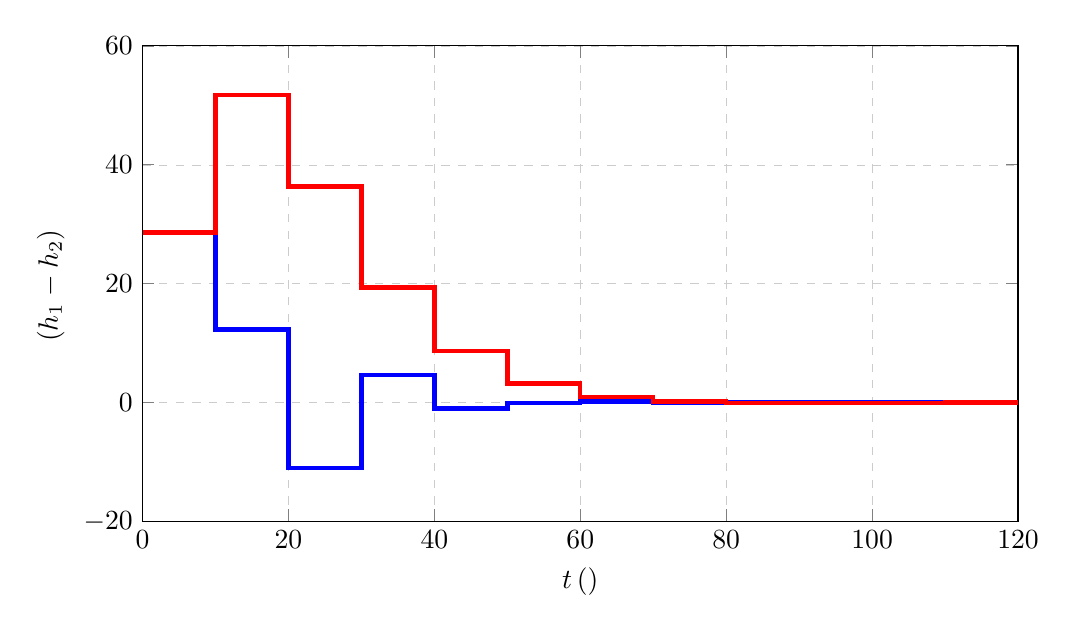
\begin{tikzpicture}

  \begin{axis}[%
    width=5in,
    height=3in,
    xlabel=$t\,(\si{\second})$,
    ylabel={$(h_1-h_2)$\,\si{\milli\metre}},
    xmin=0,
    xmax=120,
    ymin=-0.02,
    ymax=0.06,
    scaled y ticks=manual:{}{\pgfmathparse{#1*1e3}},
    xtick distance=20,
    grid=major,
    grid style={dashed, gray!40, ultra thin}
    ]
\addplot [color=blue, ultra thick, forget plot]
  table[row sep=crcr]{%
0	0.0285714285714286\\
10	0.0285714285714286\\
10	0.0122448979591837\\
20	0.0122448979591837\\
20	-0.0110787172011662\\
30	-0.0110787172011662\\
30	0.00458142440649729\\
40	0.00458142440649729\\
40	-0.00103528291783186\\
50	-0.00103528291783186\\
50	-6.28989621671243e-05\\
60	-6.28989621671243e-05\\
60	0.000183839823785765\\
70	0.000183839823785765\\
70	-9.6065761853705e-05\\
80	-9.6065761853705e-05\\
80	2.8631889089865e-05\\
90	2.8631889089865e-05\\
90	-2.63739921510786e-06\\
100	-2.63739921510786e-06\\
100	-2.58318460420479e-06\\
110	-2.58318460420479e-06\\
110	1.85287680456101e-06\\
120	1.85287680456101e-06\\
120	-6.89760373434176e-07\\
};

\addplot [color=red, ultra thick, forget plot]
  table[row sep=crcr]{%
0	0.0285714285714286\\
10	0.0285714285714286\\
10	0.0517102241391118\\
20	0.0517102241391118\\
20	0.0363211588315332\\
30	0.0363211588315332\\
30	0.0193580082941813\\
40	0.0193580082941813\\
40	0.00861324112790829\\
50	0.00861324112790829\\
50	0.0032106196542664\\
60	0.0032106196542664\\
60	0.00092498196037596\\
70	0.00092498196037596\\
70	0.000124680065202577\\
80	0.000124680065202577\\
80	-7.89238511857013e-05\\
90	-7.89238511857013e-05\\
90	-8.81657536989918e-05\\
100	-8.81657536989918e-05\\
100	-5.6052063079255e-05\\
110	-5.6052063079255e-05\\
110	-2.82471087735702e-05\\
120	-2.82471087735702e-05\\
120	-1.19747442212685e-05\\
};
\end{axis}
\end{tikzpicture}%
\caption{Resposta ao impulso do sistema compensado a partir da aproximação elíptica. Em azul, encontra-se a saída do sistema não-compensado e em laranja, a saída compensada.}
\label{fig:ImpulseE}
\end{figure}

Para a aproximação elíptica, o algoritmo retorna uma solução factível (todos os resíduos referentes às restrições são positivos). É esperado devido o melhor aproveitamento da região $\omega_n$-constante. A figura \ref{fig:ImpulseE} mostra o diagrama de pólos do sistema compensado. A matriz de ganho $K$ possui o seguinte valor:

\begin{equation}
K = \left[2,5076 \enspace -0,1807\right]\label{res:GanhoE}
\end{equation}

O máximo sobressinal é de $5,17\%$, também abaixo do especificado. O tempo de acomodação também foi respeitado, conforme visto na figura \ref{fig:ImpulseE}.

\begin{figure}[!htb]
\centering
% This file was created by matlab2tikz.
%
%The latest updates can be retrieved from
%  http://www.mathworks.com/matlabcentral/fileexchange/22022-matlab2tikz-matlab2tikz
%where you can also make suggestions and rate matlab2tikz.
%
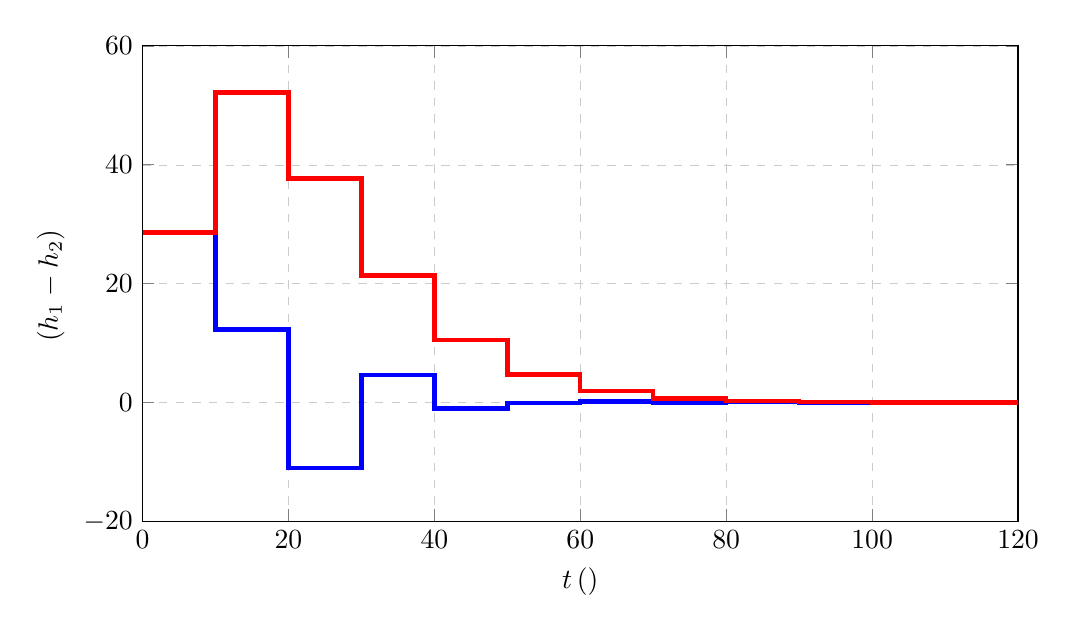
\begin{tikzpicture}

  \begin{axis}[%
    width=5in,
    height=3in,
    xlabel=$t\,(\si{\second})$,
    ylabel={$(h_1-h_2)$\,\si{\milli\metre}},
    xmin=0,
    xmax=120,
    ymin=-0.02,
    ymax=0.06,
    scaled y ticks=manual:{}{\pgfmathparse{#1*1e3}},
    xtick distance=20,
    grid=major,
    grid style={dashed, gray!40, ultra thin}
    ]
    \addplot [color=blue, ultra thick, forget plot]
    table[row sep=crcr]{%
  0	0.0285714285714286\\
  10	0.0285714285714286\\
  10	0.0122448979591837\\
  20	0.0122448979591837\\
  20	-0.0110787172011662\\
  30	-0.0110787172011662\\
  30	0.00458142440649729\\
  40	0.00458142440649729\\
  40	-0.00103528291783186\\
  50	-0.00103528291783186\\
  50	-6.28989621671243e-05\\
  60	-6.28989621671243e-05\\
  60	0.000183839823785765\\
  70	0.000183839823785765\\
  70	-9.6065761853705e-05\\
  80	-9.6065761853705e-05\\
  80	2.8631889089865e-05\\
  90	2.8631889089865e-05\\
  90	-2.63739921510786e-06\\
  100	-2.63739921510786e-06\\
  100	-2.58318460420479e-06\\
  110	-2.58318460420479e-06\\
  110	1.85287680456101e-06\\
  120	1.85287680456101e-06\\
  120	-6.89760373434176e-07\\
  };
  
  \addplot [color=red, ultra thick, forget plot]
    table[row sep=crcr]{%
  0	0.0285714285714286\\
  10	0.0285714285714286\\
  10	0.0521600797278742\\
  20	0.0521600797278742\\
  20	0.0376976130215085\\
  30	0.0376976130215085\\
  30	0.0213272628001287\\
  40	0.0213272628001287\\
  40	0.0105279983714782\\
  50	0.0105279983714782\\
  50	0.00468655046757973\\
  60	0.00468655046757973\\
  60	0.00189200469829813\\
  70	0.00189200469829813\\
  70	0.000681880644349952\\
  80	0.000681880644349952\\
  80	0.000207632156304132\\
  90	0.000207632156304132\\
  90	4.33602051682834e-05\\
  100	4.33602051682834e-05\\
  100	-3.19632114479195e-06\\
  110	-3.19632114479195e-06\\
  110	-1.07822114587915e-05\\
  120	-1.07822114587915e-05\\
  120	-8.3015346125053e-06\\
  };
\end{axis}
\end{tikzpicture}%
\caption{Resposta ao impulso do sistema compensado a partir da aproximação poligonal. Em azul, encontra-se a saída do sistema não-compensado e em laranja, a saída compensada.}
\label{fig:ImpulseP}
\end{figure}

Já para a aproximação poligonal, o algoritmo retorna uma solução factível (os resíduos associados são positivos)com duas iterações. As regiões aproximadas foram representadas na figura \ref{fig:ImpulseP} e a matriz de ganho $K$ é dado por:

\begin{equation}
K = \left[2,4159 \enspace -0,1554\right]\label{res:GanhoP}
\end{equation}

O máximo sobressinal é de $5,21\%$, também abaixo do especificado. O tempo de acomodação foi dentro do projetado.

\section{Conclusão parcial}
Com este pequeno projeto, foi possível observar o funcionamento do algoritmo e da aplicação da programação semidefinida para resolver problemas de otimização que envolvem LMIs. Em adição a isso, para a aproximaçao cônica, o solucionador numérico retorna uma solução infactível, mesmo sendo estável a solução. Vale ressaltar que nem sempre isso ocorre. Como a aproximação cônica tem uma menor área de cobertura, a região de interesse é menor, o que resulta em uma limitação para possíveis erros.

Em relação à aproximação elíptica, como a área de interesse é maior, a solução retornada é totalmente factível, o que resultou em um menor máximo sobressinal e também no tempo de acomodação.

Para a aproximação poligonal, a solução é factível, porém tem o mesmo valor para o máximo sobressinal, pois foi resolvido em duas iterações. A região aproximada tem o formato da figura \ref{fig:ImpulseP}. Como comentado para a aproximação cônica, a área coberta é menor que a da elíptica, porém maior que a da cônica, resultando em uma resposta semelhante à esta.